% ===== merged source: pages/p01.tex =====
% !TEX root = ../main.tex
\thispagestyle{empty}
\begin{center}
\vspace*{22mm}
{\Large 金融人工智能大赛\par}
\vspace{20mm}
{\Huge\bfseries 低空智研\par}
\vspace{7mm}
{\Large 低空经济产业链投研智能体\par}
\vspace{12mm}
{\LARGE 项目计划书\par}
\vspace{14mm}
{\large SkyNexus\par}
\vspace{7mm}
计划书撰写：吕洪宇、武桐宇\par
\vspace{7mm}
版本：项目计划书初稿 V1\quad 日期：\today\par
\end{center}
\vfill
\begin{center}\small
以“事件—产业路径—公司—财务—证据”为主线的可追溯研究工作台
\end{center}


% ===== merged source: pages/p02.tex =====
% !TEX root = ../main.tex
\clearpage
\tableofcontents


% ===== merged source: pages/p03.tex =====
% !TEX root = ../main.tex
\clearpage
\section{项目概要}
\subsection*{1.1 研究问题}\label{page:03}
\noindent\textbf{低空经济投研的核心任务，是把政策、材料价格、企业公告等事件转化为能够逐层审阅的产业与公司研究。}低空产业横跨航空器制造、动力系统、复合材料、空域基础设施、运营服务等环节。同一事件进入不同环节后，会经由成本、供给、订单、合规与运营效率等机制形成不同的经济含义。高质量研究必须同时回答三个决定性问题：事件事实是否可靠，传导路径如何成立，公司结论由哪些可定位证据支撑。

传统人工研究往往在公告、政策原文、行业报告和财务资料之间往返：先识别事件，再推断受影响环节，再寻找相关公司，最后补充财务解释。低空智研将这套经验性流程沉淀为统一记录，使事件、数据版本或公司映射更新后，研究者仍能沿同一结构逐段更新结论。通用问答系统擅长加速阅读；本项目进一步将事件识别、关系判断、财务解释和证据引用拆分为可组合对象，使来源、适用条件和计算口径始终随报告保留。

本项目将问题界定为\textbf{事件驱动的低空产业链投研编排任务}：给定具有来源、日期和方向的事件对象，系统沿产业知识图谱组织传导路径；对具有显式证券代码的公司映射计算影响强度；再将结论、路径和公司逐一绑定到可定位的证据。最终交付是一份包含事件ID、数据版本、路径ID、公司代码、评分字段、证据ID与运行记录的结构化报告。报告中的任一结论均可回到其事件、关系、公司和证据层重新审阅\cite{lhy-architecture,lhy-contracts}。

以仓库中已实现的“动力电池价格下降15\%”示例为例，研究对象首先被登记为唯一事件标识；总控据此读取\texttt{mock-v1}版本的事件、路径、公司、评分和证据输入，形成从电池材料到电推进、eVTOL整机与运营场景的业务ID路径。该案例完整展示了研究对象如何被传递、校验和呈现：数据版本定义分析范围，路径关系承载产业传导，评分字段表达公司影响，证据与运行记录共同构成报告的审阅入口\cite{lhy-repository,lhy-frontend}。

\begin{center}\small 表3-1\quad 投研问题、结构化对象与审阅入口的对应关系\par\vspace{1mm}
\begin{tabularx}{\linewidth}{p{0.19\linewidth}p{0.28\linewidth}X}
\toprule
研究问题 & 必须固定的研究对象 & 审阅者可以回查的内容\\
\midrule
发生了什么、何时发生 & \texttt{event\_id}、事件类型、日期、方向、来源与核验状态 & 事件卡、来源标题与链接、数据版本、运行时间\\
影响经由何处传导 & 有序节点ID、关系ID、规则ID、方向与适用条件 & 每一跳的上下游关系、路径长度、路径证据与规则说明\\
为什么关注特定公司 & 证券代码、产业角色、暴露度、敏感度、财务重要性与风险标记 & 公司--产品--节点映射、分数构成、公司证据ID与核验状态\\
结论是否可重放 & 报告ID、\texttt{run\_id}、输入版本、公式版本与错误状态 & 运行记录、接口响应、评分复算结果与异常原因\\
\bottomrule
\end{tabularx}\end{center}


% ===== merged source: pages/p04.tex =====
% !TEX root = ../main.tex
\subsection*{1.2 项目基础}\label{page:04}
\noindent\textbf{低空智研已经形成“结构化输入—确定性编排—可审阅报告”的完整研究闭环。}后端总控按注册版本读取事件、产业路径、公司映射、财务评分和证据五类输入；服务层将结果以稳定接口返回；前端以同一份报告呈现事件、路径、公司、分数、来源和运行信息。该设计使数据资产持续扩展，研究记录始终保持一致：Mock样例、审核后的行业数据库与模型辅助抽取的候选记录均通过同一份契约和核验规则进入主链\cite{lhy-architecture,lhy-orchestrator}。

\begin{center}
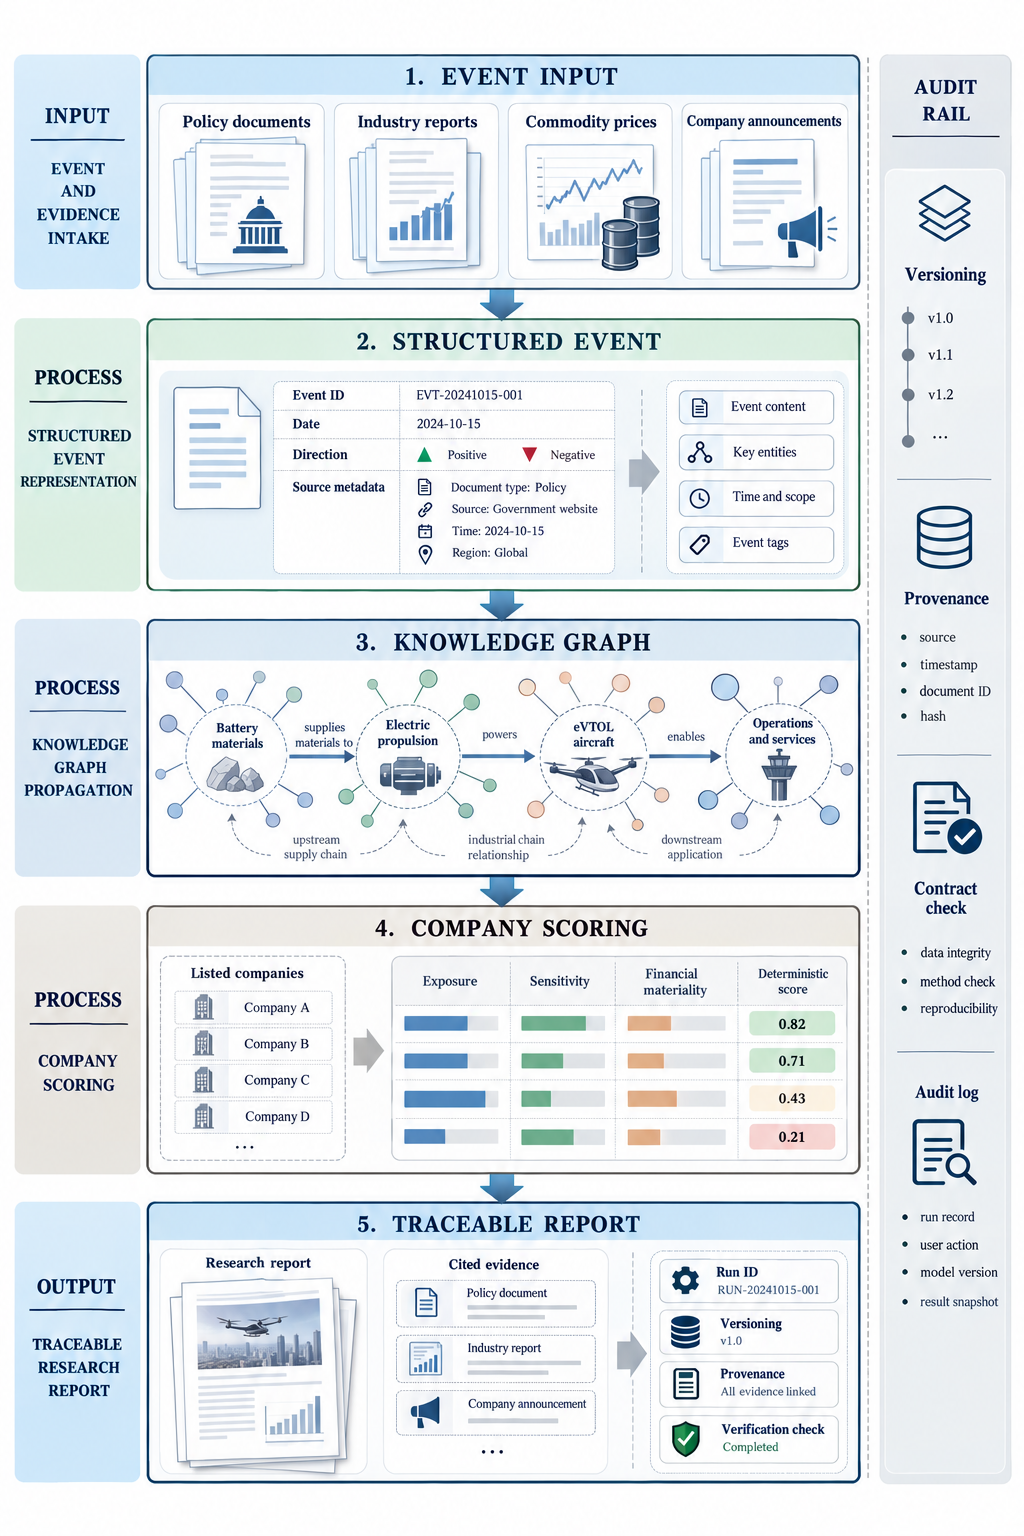
\includegraphics[width=0.88\linewidth,height=0.48\textheight,keepaspectratio]{assets/hongyulyu714-prog/fig-research-architecture.png}
\PlanFigureCaption{图4-1}{低空智研的事件驱动研究架构。图中从上至下依次呈现事件与证据输入、事件结构化、产业图谱传导、公司影响评分与可追溯报告；右侧审计轨道对应数据版本、来源、契约校验和运行记录。该图为本项目方法结构图，具体系统界面见图9--13。}
\end{center}

图4-1呈现的重点，是模块之间的严密约束。事件层负责确定研究问题的时间、方向和来源；产业图谱层把“相关”拆解为可逐段核对的节点与关系；公司评分层把暴露度、传导敏感度和财务重要性以确定性计算保留；证据与运行层为输出提供来源、版本与可复跑入口。五类对象共同形成报告的研究骨架，使同一份输出同时服务于研究阅读、代码测试和赛题答辩。

\noindent\textbf{本项目的核心贡献，是将事件、产业路径、公司、财务解释和证据约束到同一条可追溯研究链中。}已有工作已提供确定性总控、结构化接口、前端研究工作台及独立图谱、证据、评分资产；后续工作围绕统一契约完成数据接入与事件级评测。由此，研究者不必在“看见一个结论”和“找到结论依据”之间反复切换，评审也能以同一套结构检查系统检查事实基础、推理过程和输出边界。

\begin{center}\small 表4-1\quad 已形成资产、当前状态与其在主链中的角色\par\vspace{1mm}
\begin{tabularx}{\linewidth}{p{0.21\linewidth}p{0.18\linewidth}X}
\toprule
资产或能力 & 当前状态 & 已有证据与使用口径\\
\midrule
确定性总控与接口契约 & 已实现、已测试 & 接收五类结构化输入，检查ID、证券代码、路径关系数、评分范围与证据引用；默认注册版本为\texttt{mock-v1}。\\
研究工作台与报告阅读 & 已实现、已测试 & 已支持事件选择、分析请求、业务ID路径、公司比较、证据抽屉、来源与运行信息的连续阅读。\\
产业图谱数据包 & 已交付、接入中 & 独立数据包含35个节点、50条关系、25项公司映射和10条事件规则，是事件级传导分析的结构化基础。\\
评分样例与方法文档 & 可复现、Mock输入 & 20家临时研究对象、3类情景、60条评分与240条财务样例行，用于检验公式、单位、缺失值和展示逻辑。\\
事件证据与评测资产 & 已交付、接入中 & 已整理30条事件、31条证据片段和30道评测题，用于事件级检索、引用核验和效果评测。\\
自动化验证记录 & 已记录 & 前端31项单元测试、20个Linux Chrome场景、后端37项测试，以及类型检查、Lint、构建与三平台CI记录。\\
\bottomrule
\end{tabularx}\end{center}
\SourceNote{数量、状态和验证口径来自项目README、架构文档、图谱说明、评分方法、证据复核说明与前端演示文档；访问日期：2026-10-15。}

这些成果共同构成了后续评测的可操作起点。工程闭环已有明确的运行与测试记录；图谱、证据和评分资产已具备独立的数据结构与来源说明；接下来的集成工作将以事件ID和数据版本为锚，把它们接入同一报告主链，并用固定任务集检验路径正确性、证据可定位性和公司研究队列质量。项目由工程运行、事件研究和用户任务三类证据共同支撑：前者确认报告生成链路，第二类确认事件传导与公司解释，第三类确认研究者可以据此完成可复核的分析任务。


% ===== merged source: pages/p05.tex =====
% !TEX root = ../main.tex
\clearpage
\section{行业问题与用户需求}
\subsection*{低空产业与金融研究对象}\label{page:05}
\ifdraftversion{\noindent\small\color{gray}写作页位 5\quad 负责人 武桐宇\par}\fi
\WritingGuide{解释材料、动力、控制、整机、设施和运营之间的关系。}{产业链全景图及来源。}{产业规模等外部数字须保留时间与统计口径。}
\NeedEvidence{替换本页写作指引，补入正文、真实材料与可定位出处。}
\FigureSlot{低空产业与金融研究对象所需图表}{产业链全景图及来源。}

% 按“一句话结论—证据—解释—适用条件”组织本页正文。


% ===== merged source: pages/p06.tex =====
% !TEX root = ../main.tex
\PlanPage{现有投研流程与具体困难}{武桐宇}{06}
\WritingGuide{梳理资料查询、公司匹配、财务核对和结果复核的任务。}{现有流程和问题证据。}{不以无来源的行业痛点替代需求调查。}
\NeedEvidence{替换本页写作指引，补入正文、真实材料与可定位出处。}
\FigureSlot{现有投研流程与具体困难所需图表}{现有流程和问题证据。}

% 按“一句话结论—证据—解释—适用条件”组织本页正文。


% ===== merged source: pages/p07.tex =====
% !TEX root = ../main.tex
\PlanPage{目标用户与典型场景}{武桐宇}{07}
\WritingGuide{区分高校研究、机构投研和产业研究，确定首批用户。}{用户、任务频率、交付形式比较表。}{潜在客户、访谈对象和已合作客户分开。}
\NeedEvidence{替换本页写作指引，补入正文、真实材料与可定位出处。}
\FigureSlot{目标用户与典型场景所需图表}{用户、任务频率、交付形式比较表。}

% 按“一句话结论—证据—解释—适用条件”组织本页正文。


% ===== merged source: pages/p08.tex =====
% !TEX root = ../main.tex
\PlanPage{需求验证与评价标准}{武桐宇}{08}
\WritingGuide{把用户需求转为可检查的产品要求。}{访谈记录或拟开展的调研方案。}{没有实际访谈时不得虚构引语与反馈。}
\NeedEvidence{替换本页写作指引，补入正文、真实材料与可定位出处。}
\FigureSlot{需求验证与评价标准所需图表}{访谈记录或拟开展的调研方案。}

% 按“一句话结论—证据—解释—适用条件”组织本页正文。


% ===== merged source: pages/p09.tex =====
% !TEX root = ../main.tex
\clearpage
\section{产品设计与使用流程}
\subsection*{3.1 研究工作台}\label{page:09}
\noindent\textbf{低空智研以事件驱动研究工作台组织投研流程。}研究者从一个已登记事件出发，在同一研究现场依次阅读事件事实、产业传导路径、公司比较、评分构成、证据摘录和运行来源。界面将这些对象置于一份报告上下文中，使使用者能够沿结论反向检查：某家公司为何出现在研究队列中、该公司受到何种方向的影响、系统依据了哪条路径、引用来自何处。

\begin{center}
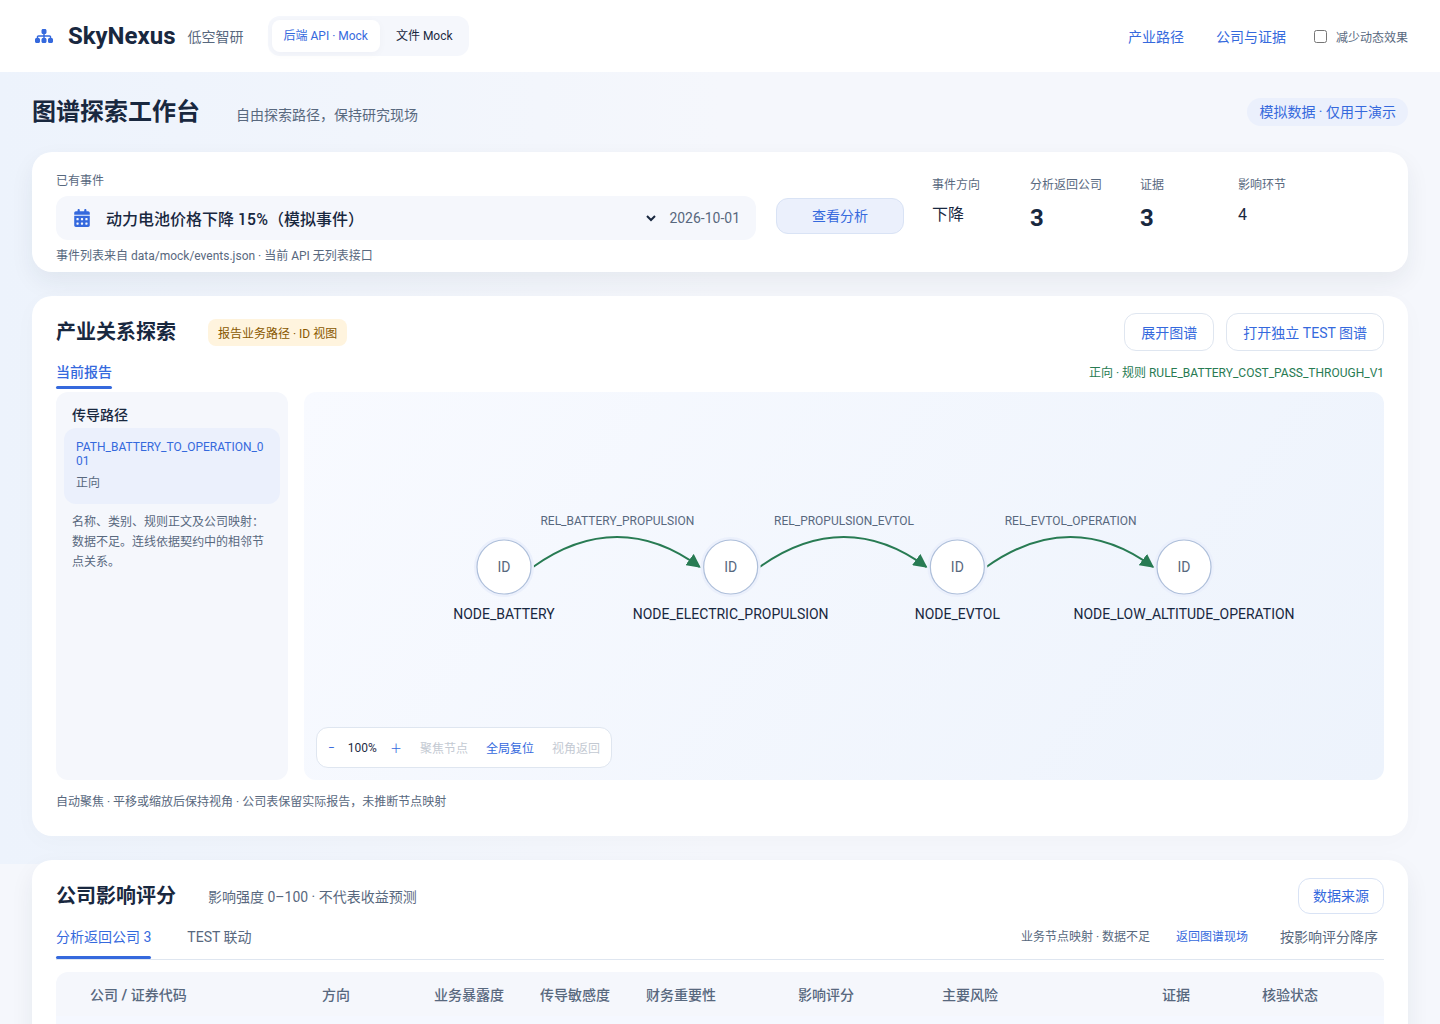
\includegraphics[width=0.94\linewidth,height=0.43\textheight,keepaspectratio]{assets/hongyulyu714-prog/fig-workbench.png}
\PlanFigureCaption{图9-1}{当前业务工作台截图。页面在“后端API·Mock”模式下展示已选事件、业务图谱、公司影响、证据抽屉和研究现场；截图来源于仓库\texttt{docs/screenshots/03-business-1440.png}，采集清单记录的实现提交为\texttt{86a440a}。}
\end{center}

图9-1所示界面将“得到答案”转化为“完成研究动作”。研究者先确认事件与版本，再主动提交分析；返回报告后，先阅读图谱中的有序业务ID，再查看与路径相关的公司卡片；随后通过证据抽屉、来源与运行信息完成复核。页面排序、路径阅读、公司比较和证据回溯共同构成具备对象层次的研究证据索引\cite{lhy-frontend,lhy-architecture}。

\begin{center}\small 表9-1\quad 工作台的研究动作、输出对象与使用价值\par\vspace{1mm}
\begin{tabularx}{\linewidth}{p{0.20\linewidth}p{0.30\linewidth}X}
\toprule
研究动作 & 页面输出对象 & 对投研工作的价值\\
\midrule
选择并确认事件 & 事件名称、\texttt{event\_id}、来源、方向、版本与状态 & 将研究对象固定在明确的时间和来源口径内，避免不同模块围绕相似文本分别理解。\\
发起一次分析 & 报告ID、\texttt{run\_id}、生成时间、数据版本和异常状态 & 让每次研究请求成为可重放的记录，而非一次性的页面刷新。\\
阅读产业路径 & 节点ID、关系ID、方向、规则入口和路径证据 & 将“产业相关”展开为一系列可逐边核验的传导命题。\\
比较公司影响 & 证券代码、角色、方向、影响分、风险标记和证据ID & 把公司筛选从概念罗列推进为可审阅的候选研究队列。\\
打开证据与来源 & 标题、日期、摘录、URL、可信度、核验状态与运行信息 & 支持研究者回到原始材料，检验结论是否超出证据的支持范围。\\
\bottomrule
\end{tabularx}\end{center}
\SourceNote{当前前端能力、模式与截图口径来自\texttt{docs/FRONTEND\_DEMO.md}及其截图清单；访问日期：2026-10-15。}

产品设计的重点在于保持研究链的连续性。事件、路径、公司、评分和证据在数据层上分别管理，在阅读层上却被组织为一条可追溯的论证链；这既减少了研究者跨文件寻找依据的成本，也使后续替换数据源时可以准确识别报告中的变化来自事件、图谱、财务还是证据层。当前工作台使用已登记的Mock事件验证这一交互闭环，随后将承接通过审核的数据版本和真实事件级评测。


% ===== merged source: pages/p10.tex =====
% !TEX root = ../main.tex
\subsection*{3.2 事件入口}\label{page:10}
\noindent\textbf{事件入口在分析开始前将研究对象转化为具有时间、方向、来源和版本的结构化记录。}金融研究中的“事件”需要明确发生或披露的日期、影响对象、方向、材料来源与核验状态，才能在图谱、公司、财务和证据模块中保持同一语义。研究者选择已登记事件后，前端将事件ID与数据版本提交给总控，由总控调度后续研究任务。

\begin{center}
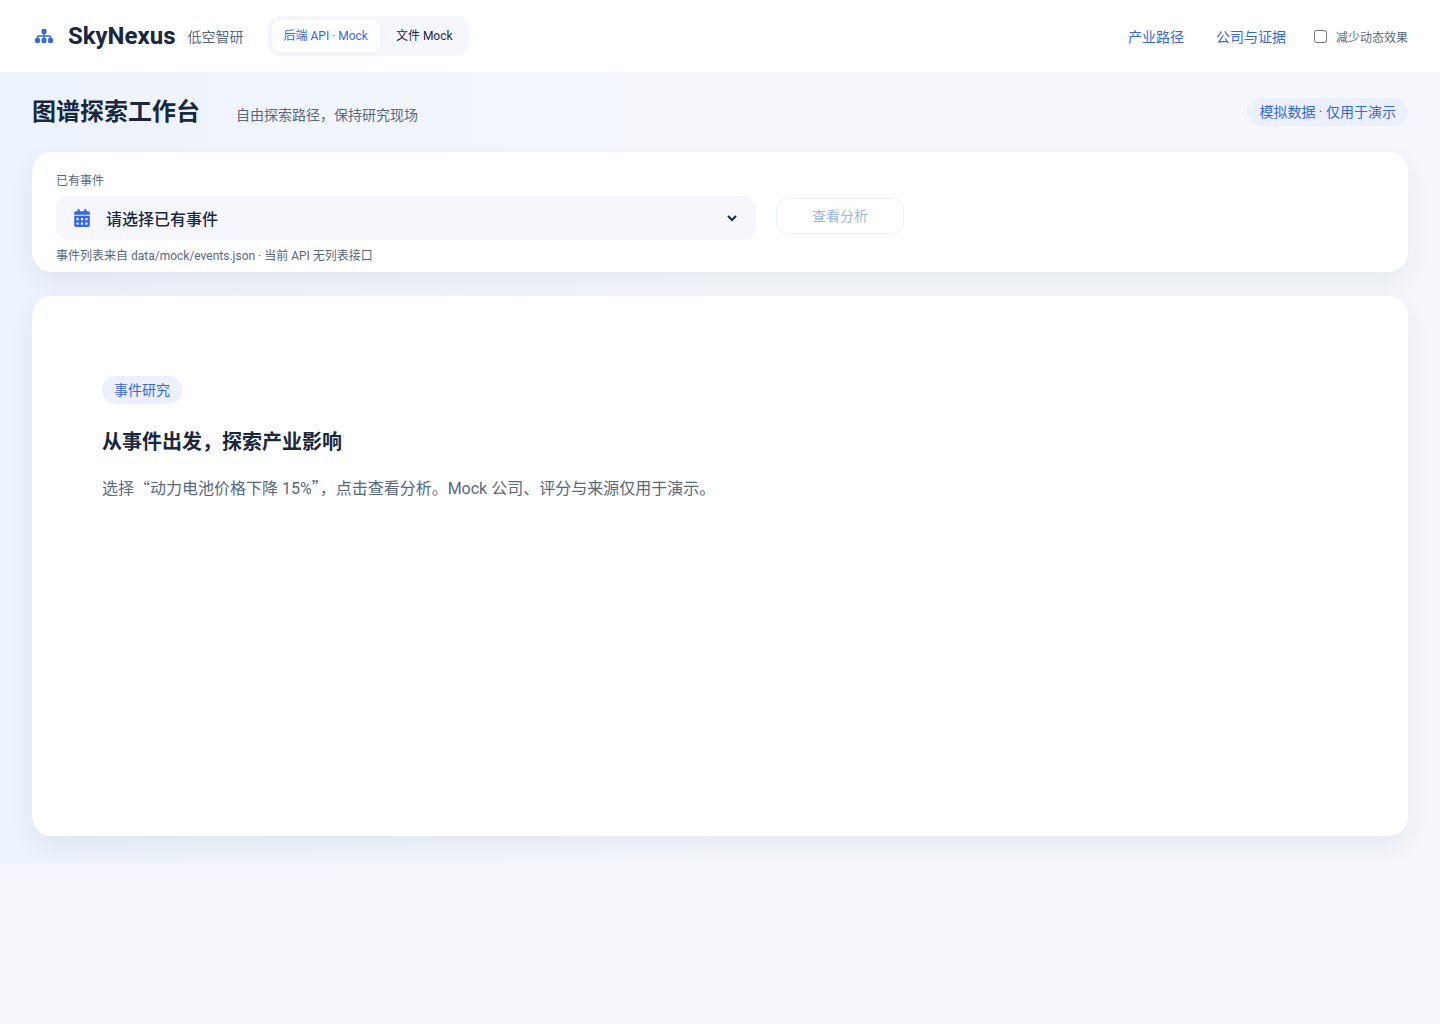
\includegraphics[width=0.88\linewidth,height=0.37\textheight,keepaspectratio]{assets/hongyulyu714-prog/fig-event-entry.png}
\PlanFigureCaption{图10-1}{事件入口截图。工作台展示当前事件选择和分析按钮；截图来源于仓库\texttt{docs/screenshots/01-entry.png}。当前事件池服务于Mock全链路验证，研究者在发起分析前能够确认事件名称与模式。}
\end{center}

对于任何拟接入的事件，系统首先建立事件卡：\texttt{event\_id}承担跨模块主键功能，事件名称与类型定义研究主题，日期与方向限定时间语境和作用方向，受影响节点为图谱查询设定起点，来源标题、URL与核验状态为后续事实审阅保留入口。只有当这些字段随同事件进入总控，报告中的路径、公司、分数和证据才可以被识别为围绕同一个研究对象生成\cite{lhy-contracts,lhy-architecture}。

\begin{center}\small 表10-1\quad 事件对象的字段设计及其在研究链中的作用\par\vspace{1mm}
\begin{tabularx}{\linewidth}{p{0.19\linewidth}p{0.26\linewidth}X}
\toprule
字段组 & 在系统中的作用 & 研究审阅时应回答的问题\\
\midrule
唯一标识 & \texttt{event\_id}连接路径、公司、评分、证据和运行记录 & 这些对象是否确实属于同一事件，而非来自相似但不同的行业新闻？\\
事实描述 & 名称、类型、日期、地区、方向与受影响节点定义研究范围 & 事件究竟改变了什么，变化发生在哪个时间与产业环节？\\
来源信息 & 标题、URL、发布日期、摘录与核验状态保留事实定位 & 研究者能否回到原始材料，确认当前表述没有超出来源？\\
版本信息 & \texttt{data\_version}约束本次运行使用的一组数据资产 & 报告中的路径、评分和证据是否来自可识别且相互兼容的版本？\\
运行信息 & \texttt{run\_id}、开始/结束时间、状态与错误文本记录分析过程 & 同一输入是否可重放；若失败，失败发生在何处？\\
\bottomrule
\end{tabularx}\end{center}

事件被提交后，总控首先登记一次运行，再读取对应版本的五类输入，完成事件、路径、评分与证据的协同组织\cite{lhy-orchestrator}。这条流程使事件识别、数据治理与分析启动成为同一件事：研究对象一旦变化，后续所有推理均以新的事件记录和新运行记录为准。自然语言解析将作为候选事件发现模块接入，其输出经来源、字段、版本与人工复核后进入研究主链。


% ===== merged source: pages/p11.tex =====
% !TEX root = ../main.tex
\subsection*{3.3 产业路径}\label{page:11}
\noindent\textbf{在事件驱动投研中，产业路径用于解释影响如何从一个环节传递至下一个环节。}低空智研将路径定义为有序节点ID和相邻关系ID组成的\texttt{GraphPath}：节点给出材料、部件、整机或运营环节；关系给出供应、配套、驱动或服务等方向；规则和证据说明关系的适用条件。接口要求一条路径的关系数量等于节点数量减一，使每条边均可对应其前后节点\cite{lhy-contracts}。

\begin{center}
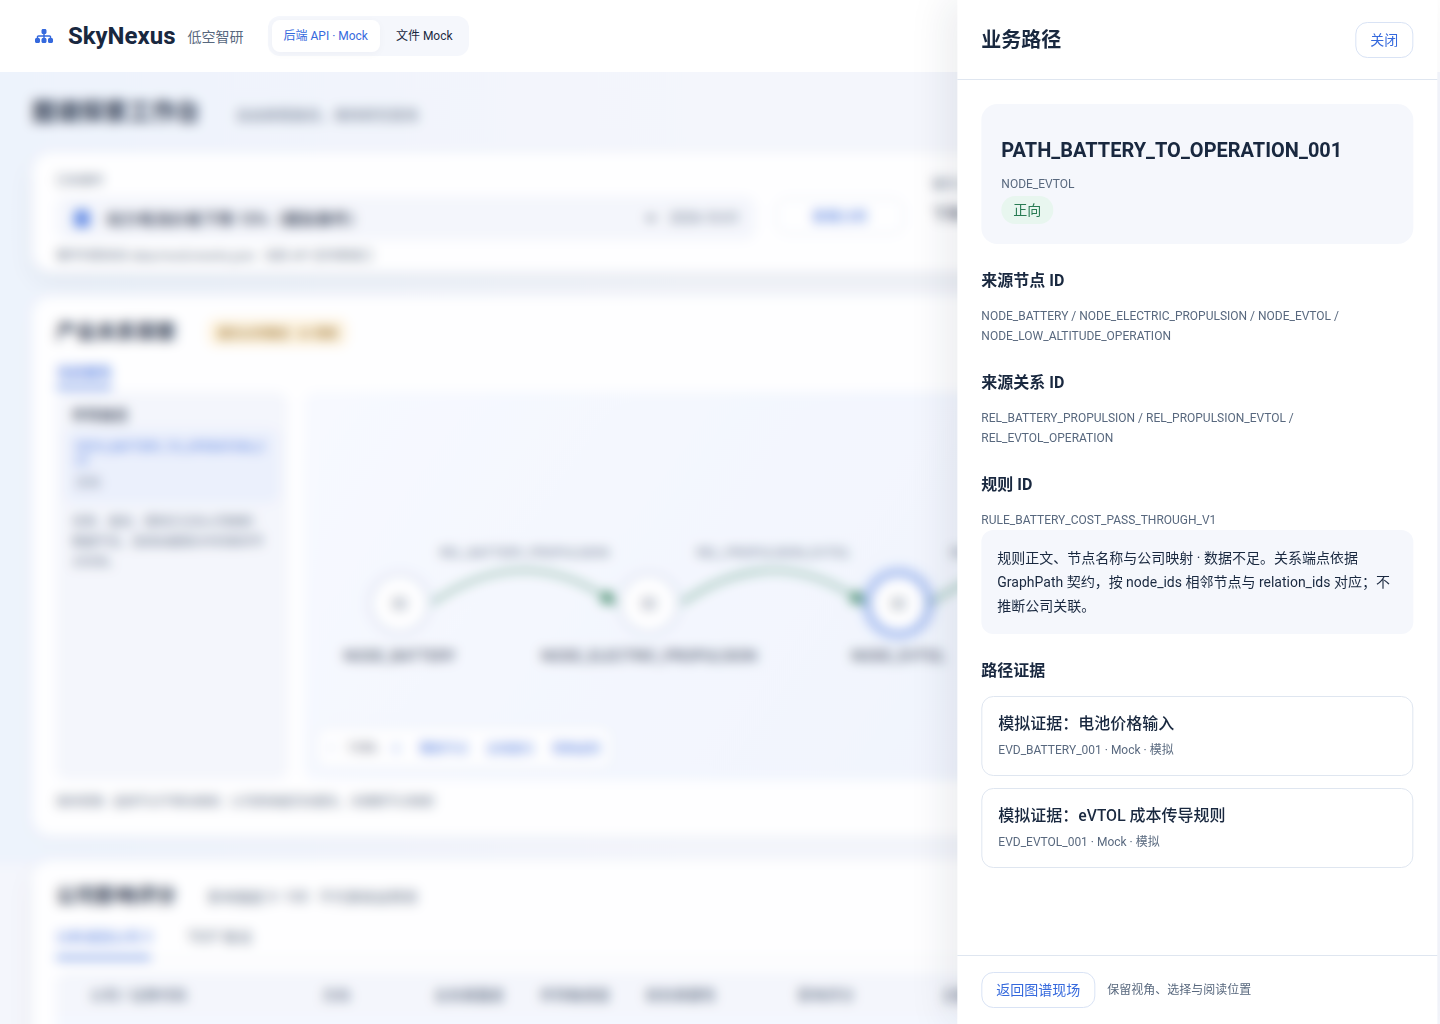
\includegraphics[width=0.90\linewidth,height=0.39\textheight,keepaspectratio]{assets/hongyulyu714-prog/fig-path-evidence.png}
\PlanFigureCaption{图11-1}{路径规则与证据阅读截图。图中展示业务ID路径的节点选择、规则标识和证据入口；截图来源于\texttt{docs/screenshots/06-business-path.png}。界面重点呈现关系链及其审阅入口，而非以节点数量制造复杂度。}
\end{center}

以电池价格变化为例，项目将传导展开为多个可以独立核对的命题：电池材料或电芯成本的改变如何作用于电推进系统；电推进系统如何嵌入eVTOL整机；整机成本、性能或交付条件又如何影响下游运营。每一跳均由关系、适用条件和证据支撑，研究者能够从具体技术和业务关系出发形成经济解释。这种层级化表达使产业研究具备可阅读、可讨论、可复核的中间层。

\begin{center}\small 表11-1\quad 产业传导路径的四个审阅层次\par\vspace{1mm}
\begin{tabularx}{\linewidth}{p{0.16\linewidth}p{0.30\linewidth}X}
\toprule
审阅层次 & 需要确认的内容 & 系统保留的结构化信息\\
\midrule
节点层 & 事件首先影响的是材料、部件、整机还是运营场景？ & \texttt{node\_id}、节点类型、节点名称或别名、所属产业环节。\\
关系层 & 两个相邻节点之间是否存在明确的业务或技术连接？ & \texttt{relation\_id}、关系类型、方向与路径中的前后位置。\\
规则层 & 该连接在何种条件下成立，可能受到哪些边界约束？ & 规则ID、规则说明、适用范围、数据状态与缺失提示。\\
证据层 & 该路径的事实基础可以由哪一份来源材料定位？ & \texttt{evidence\_ids}、来源标题、日期、摘录、URL和核验状态。\\
经济解释层 & 技术或业务连接如何转化为成本、收入或风险的研究命题？ & 公司角色、影响方向、评分构成与附加财务解释，避免由技术连接直接推出投资结论。\\
\bottomrule
\end{tabularx}\end{center}

仓库的独立产业图谱数据包已整理35个节点、50条关系、25项公司映射和10条事件规则，为后续事件级查询提供了可审计资产\cite{lhy-graph}。当前报告API展示的为Mock业务ID路径，图谱数据包将通过相同契约接入主链。把业务路径、交互测试图谱和独立图谱资产分开标记，能使评审清楚看到当前已运行的研究路径、已交付的数据资产及其后续整合方式。


% ===== merged source: pages/p12.tex =====
% !TEX root = ../main.tex
\subsection*{3.4 公司比较}\label{page:12}
\noindent\textbf{公司比较模块将产业概念转化为可以逐项审阅的研究队列。}每个公司对象同时携带证券代码、产业角色、影响方向、影响强度、风险标记、证据ID与核验状态。公司通过证券主体、产品或业务角色与图谱节点和事件路径建立显式映射；在此基础上，系统进一步刻画该公司对事件的暴露、敏感性和财务重要性。

\begin{center}
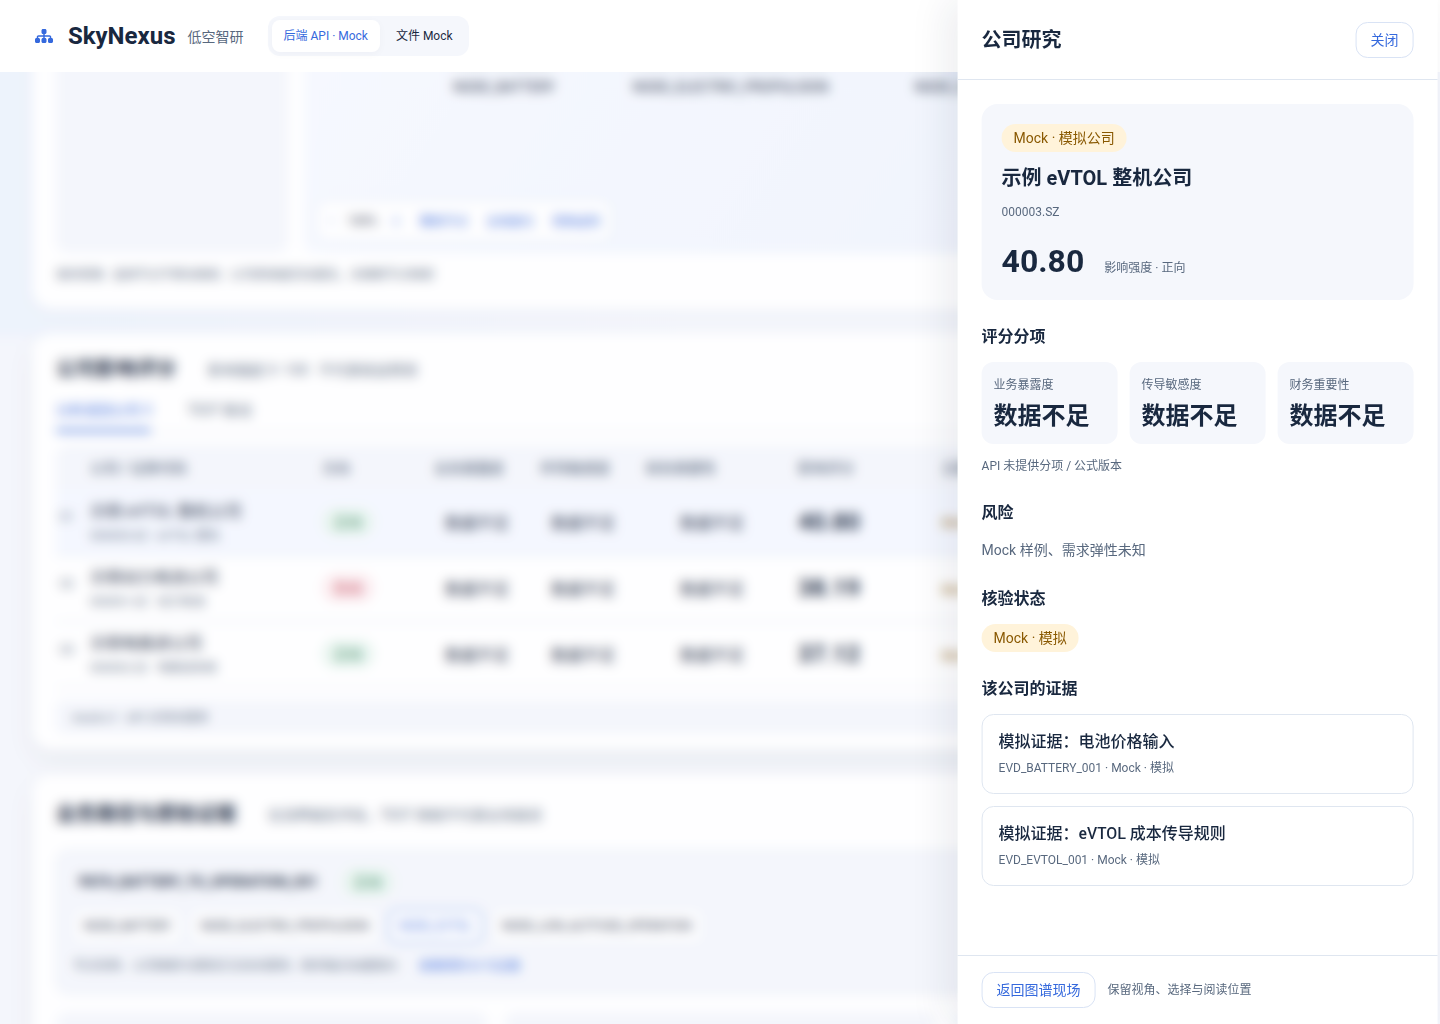
\includegraphics[width=0.90\linewidth,height=0.40\textheight,keepaspectratio]{assets/hongyulyu714-prog/fig-company-analysis.png}
\PlanFigureCaption{图12-1}{公司影响分析页面截图。页面将公司卡片、影响方向、分数、风险标记与证据入口放入同一研究现场；截图来源于\texttt{docs/screenshots/08-company.png}。图中数值属于\texttt{mock-v1}演示记录，用于展示字段和阅读路径。}
\end{center}

项目采用确定性影响强度表达式
\[
\mathrm{Impact}=\frac{\mathrm{Exposure}\times\mathrm{Sensitivity}\times\mathrm{FinancialMateriality}}{10000}.
\]
其中，\textit{Exposure}衡量公司业务与被影响产业环节的连接程度，\textit{Sensitivity}描述事件变化对该环节的传导敏感度，\textit{FinancialMateriality}表达成本、毛利、现金流或杠杆等财务变量对传导的放大程度。影响方向通过\texttt{positive}、\texttt{negative}、\texttt{neutral}和\texttt{uncertain}字段单独呈现，使研究者能够同时阅读传导方向、影响强度与风险信号\cite{lhy-scoring,lhy-architecture}。

\begin{center}\small 表12-1\quad 公司研究队列的字段、解释任务与审阅规则\par\vspace{1mm}
\begin{tabularx}{\linewidth}{p{0.20\linewidth}p{0.28\linewidth}X}
\toprule
字段组 & 回答的研究问题 & 审阅规则\\
\midrule
主体与产业角色 & 研究对象是否为明确的上市主体，位于何种业务环节？ & 使用显式证券代码和公司--产品--节点映射；概念、传闻或名称相似性不构成主体识别。\\
暴露度与敏感度 & 该公司为何会受到事件影响，影响沿何种机制传递？ & 每个参数应能追溯至产业角色、路径关系或已记录的业务事实。\\
财务重要性 & 事件传导为何可能在财务层被放大或缓冲？ & 当前为可复现代理变量；接入授权数据后按报告期、单位和口径复核。\\
方向、分数与风险 & 影响的方向、相对强度与不确定性如何共同表达？ & 方向与强度分别读取；风险标记不被压缩进单一总分。\\
证据与核验状态 & 支撑公司关联的依据是否已定位和复核？ & 证据需显式包含该证券代码；无直接关联时保留待核验状态。\\
\bottomrule
\end{tabularx}\end{center}

当前评分样例覆盖20家临时研究对象、3类事件情景和60条评分记录，并配套240条财务样例行\cite{lhy-scoring}。这些数据的作用是复现影响计算、检查单位和缺失值处理、验证前端展示，而不是替代授权财务数据库。正式比赛演示将以“公司主体可追溯、方向可解释、分数可复算、证据可定位”为评价重点，使公司比较成为研究的起点而非结论终点。


% ===== merged source: pages/p13.tex =====
% !TEX root = ../main.tex
\subsection*{3.5 证据阅读}\label{page:13}
\noindent\textbf{证据模块为每一份研究报告提供“从结论返回原始材料”的通道。}系统将一段可定位的文本摘录作为最小证据单元，记录\texttt{evidence\_id}、事件ID、来源标题、发布日期、URL、原文定位、短摘录、显式证券代码、可信度等级与核验状态。路径、公司、评分和报告结论通过证据ID获得共同的事实基础\cite{lhy-contracts,lhy-evidence}。

\begin{center}
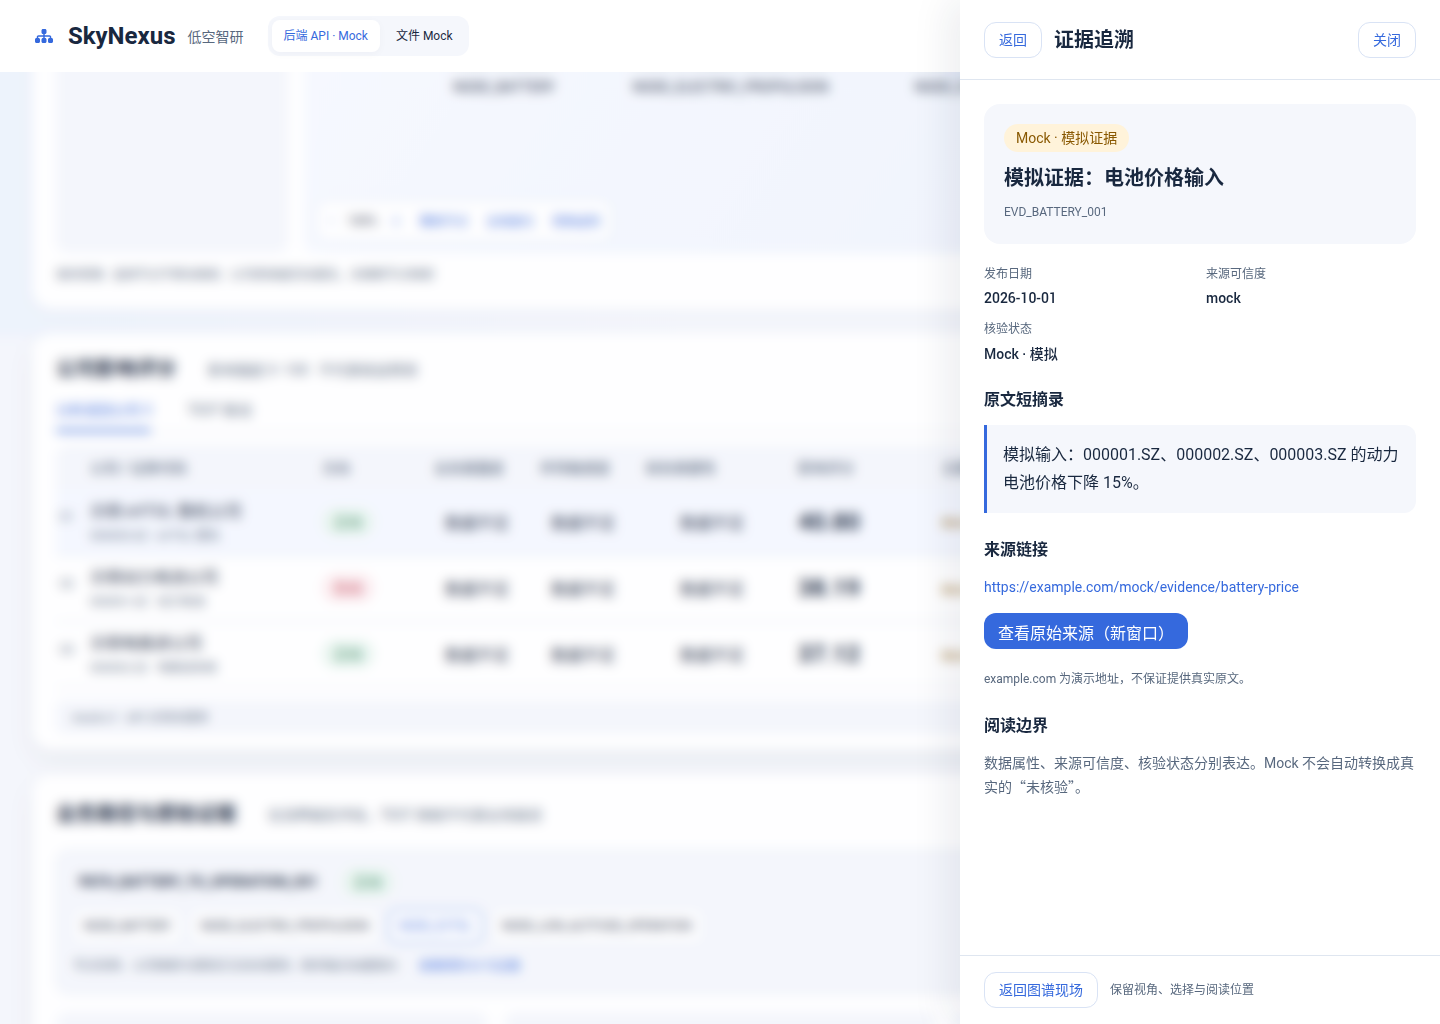
\includegraphics[width=0.88\linewidth,height=0.40\textheight,keepaspectratio]{assets/hongyulyu714-prog/fig-evidence-drawer.png}
\PlanFigureCaption{图13-1}{证据抽屉截图。使用者可在研究现场打开某条证据，阅读标题、日期、摘录、可信度与来源入口；截图来源于\texttt{docs/screenshots/09-evidence.png}。截图中的Mock状态、示例链接和核验标签均随记录展示。}
\end{center}

证据阅读将报告组织为三个层次：首先确认来源文本陈述的事实；其次识别该事实所支持的产业关系或公司映射；最后形成与证据范围一致的研究结论。以价格变化材料为例，事件事实、公司主体、产业角色和路径关系共同构成公司研究依据。三层结构使新闻、规则、公司与结论各自拥有清晰的位置，也使研究者能够在需要时快速回到原始材料。

\begin{center}\small 表13-1\quad 证据状态、报告表述与研究动作\par\vspace{1mm}
\begin{tabularx}{\linewidth}{p{0.18\linewidth}p{0.32\linewidth}X}
\toprule
记录状态 & 报告可以展示的内容 & 研究者应执行的动作\\
\midrule
可定位公开来源 & 标题、日期、URL、定位短摘录、来源等级和所支持的事实 & 回到原文核对时间、主体与上下文，再判断是否足以支持路径或公司结论。\\
已核验关联 & 证据ID、证券代码、事件/路径关联、核验状态与复核记录 & 可以作为报告中相应关联的审阅依据，并在新版本运行时重新检查。\\
Mock演示记录 & Mock标题、示例URL、Mock可信度和Mock核验状态 & 用于演示字段流、抽屉交互与引用机制；不转述为真实行业事实。\\
待核验记录 & 证据入口、风险标记与待补充事项 & 保留研究线索和下一步动作，待补齐来源或映射后重新运行报告。\\
\bottomrule
\end{tabularx}\end{center}

报告交付是一份可重放的研究成果，包含输入事件、数据版本、报告ID、\texttt{run\_id}、结构化路径、公司记录、评分构成和证据账本；新数据进入后，系统以同一事件重跑并比较变化来自何一层。前端在API模式下展示服务返回的运行信息，在文件演示模式下展示与数据包一致的研究状态\cite{lhy-frontend}。这一设计让项目以完整证据链回答“结论从何而来”的核心问题。


% ===== merged source: pages/p14.tex =====
% !TEX root = ../main.tex
\section{技术架构与智能体设计}
\subsection*{4.1 系统架构}\label{page:14}
\noindent\textbf{系统采用“研究数据模块、确定性总控、标准服务接口和研究工作台”四层架构。}事件识别、产业关系、公司映射、财务解释和证据检索具有不同的数据来源、更新频率和专业责任；项目让每一类模块先输出结构化记录，再由总控完成版本选择、字段校验、路径检查、评分复算、证据绑定和运行留痕，最终生成供API和前端消费的\texttt{Report}\cite{lhy-architecture,lhy-orchestrator}。

从数据流看，事件模块回答“本次研究什么”，图谱模块回答“影响如何传导”，公司与评分模块回答“哪些主体进入研究队列以及为什么”，证据模块回答“每项事实从何而来”。总控负责在一份报告中组织这些专业事实，确保它们使用同一事件和数据版本，并满足接口契约。模型型Agent由此进入可核对的研究结构：模型辅助抽取实体、发现候选关系和组织报告语言，输出再转写为可验证字段并接受统一检查。

\begin{center}\small 表14-1\quad 四层架构的职责边界与输入输出\par\vspace{1mm}
\begin{tabularx}{\linewidth}{p{0.17\linewidth}p{0.31\linewidth}X}
\toprule
架构层 & 核心对象与职责 & 输入、输出与审阅入口\\
\midrule
研究数据层 & 事件、路径、公司、评分与证据的标准记录；不同模块可独立更新 & 输入为经过登记的数据资产或服务结果；输出为满足JSON契约的对象及数据版本。\\
确定性总控层 & 选择同版本输入，核验跨模块引用，复算分数，形成报告与运行状态 & 输入为五类模块输出；输出为\texttt{Report}、\texttt{run\_id}、完成或失败记录。\\
服务接口层 & 向调用者提供健康检查与分析请求，隔离前端和数据存储细节 & 当前提供\texttt{GET /health}和\texttt{POST /api/v1/analyze}；输出为结构化响应与错误信息。\\
研究交互层 & 支持研究发起、路径阅读、公司比较、证据回溯和来源检查 & 输入为报告；输出为研究者可操作的图谱、卡片、证据抽屉和运行信息。\\
\bottomrule
\end{tabularx}\end{center}

该分层带来两项对金融研究特别重要的能力。其一，图谱、证据和财务数据按同一契约注册后，前端持续以事件、路径、公司、证据和运行信息的统一形态阅读。其二，数据质量控制能够定位到事件、关系、证券代码、评分或证据引用等具体层级，并以运行状态记录处理结果。研究者由此获得一份结构稳定、来源清晰、计算可复跑的投研报告。

\begin{center}\small 表14-2\quad 关键设计选择及其研究含义\par\vspace{1mm}
\begin{tabularx}{\linewidth}{p{0.26\linewidth}X}
\toprule
设计选择 & 对研究可信度与工程演进的作用\\
\midrule
以\texttt{event\_id}和\texttt{data\_version}贯穿模块 & 为同一研究对象建立主键和版本边界，避免相似事件或不同数据包在同一报告中被无意混合。\\
以显式证券代码绑定公司证据 & 将主体识别从文本猜测转化为可检查规则，使公司研究队列具有可定位的实体基础。\\
以确定性公式计算影响强度 & 让影响分可以复算、比较和回归测试；参数更新不会被隐藏在自然语言中。\\
以\texttt{run\_id}记录成功与失败运行 & 将“本次结果如何产生”保留为报告的一部分，支持复跑、排错和版本对照。\\
以界面展示数据状态与来源 & 使Mock、已核验、待核验和不同运行模式在研究阅读中保持可见，减少语义混淆。\\
\bottomrule
\end{tabularx}\end{center}
\SourceNote{架构文档、总控实现与跨模块JSON契约；访问日期：2026-10-15。}

总体而言，该架构通过数据版本、字段契约、计算规则和证据引用建立共同语言。它使低空产业研究能够在数据不断补充的条件下持续演进：新的事件、规则、公司映射或财务记录进入统一研究结构后，即可形成可审阅报告并与既有结果进行明确比较。

这一机制尤其适合低空经济的跨域研究。电池、电推进、飞行器、空域基础设施和运营服务拥有不同的知识表达、更新节奏与数据口径；统一总控将它们汇入同一份报告，同时保留各自的来源、版本与专业语义。研究者因此能够从宏观事件进入产业机制，从产业机制进入公司队列，再从公司队列进入财务解释和原始证据，形成由上而下与由下而上均可阅读的研究闭环。


% ===== merged source: pages/p15.tex =====
% !TEX root = ../main.tex
\subsection*{4.2 事件分析}\label{page:15}
\noindent\textbf{事件分析将可追溯材料转化为能够触发产业研究的规范化对象。}这一任务包含四个连续步骤：识别材料中的时间、主体、对象和变化方向；匹配预定义的研究范围；绑定来源、日期和核验状态；生成可由图谱、公司、评分与证据模块共同读取的事件记录。系统已经实现已登记事件的调用与分析，自然语言事件解析将以相同记录为输出，持续拓展事件发现能力\cite{lhy-contracts,lhy-architecture}。

事件结构化首先解决“同一事实被不同模块如何理解”的问题。例如，一条涉及电池价格变化的材料，至少需要区分价格对象、变化幅度、时间、地区、可能受影响的电池或动力系统节点，以及来源的可信度。若这些信息只被写在段落中，图谱查询、公司筛选和证据复核将分别产生不同的语义边界。相反，登记事件将事实主张、研究范围和证据入口绑定到一个\texttt{event\_id}，使后续模块围绕同一对象工作。

\begin{center}\small 表15-1\quad 事件规范化的处理单元、输出字段与质量要求\par\vspace{1mm}
\begin{tabularx}{\linewidth}{p{0.19\linewidth}p{0.30\linewidth}X}
\toprule
处理单元 & 结构化输出 & 质量要求\\
\midrule
事实抽取 & 事件名称、类型、日期、地区、方向、变化对象与幅度 & 事实描述对应原始来源定位；时间与地区以事件字段统一表达。\\
研究范围匹配 & 受影响节点、行业标签、事件类别与优先级 & 节点应使用图谱可识别的标准ID或明确的待映射状态。\\
来源绑定 & 标题、URL、发布日期、摘录、来源等级与核验状态 & 来源本身与“来源支持何种事实”同步保留，形成可定位的事实入口。\\
版本登记 & \texttt{event\_id}、\texttt{data\_version}与创建/修订信息 & 已登记版本可被复跑；后续修订形成新记录或清晰的版本关联。\\
任务触发 & 图谱查询条件、证据检索键、公司筛选范围和运行请求 & 下游模块读取事件字段，而不重新解释输入文本。\\
\bottomrule
\end{tabularx}\end{center}

事件由研究者从已登记列表选择并提交，系统据此发起分析请求。这一流程为事件对象、路径对象和报告对象之间的接口提供稳定测试条件。随着事件库和证据库接入，系统将基于统一字段扩展自然语言抽取、时空范围识别和候选关系发现；模型输出以候选结构化记录进入来源、字段和人工复核流程，随后进入正式分析。

\noindent\textbf{事件规范化让“信息出现”立即转化为可启动、可复核的研究任务。}政策文本、公告、价格材料和行业报告经由统一事件对象进入主链，产业路径、公司比较和财务解释共享同一个事实起点，从而使全链报告具备一致的可追溯性。


% ===== merged source: pages/p16.tex =====
% !TEX root = ../main.tex
\subsection*{4.3 图谱分析}\label{page:16}
\noindent\textbf{产业图谱承担“传导假设的结构化表达”功能。}给定一个事件，系统先定位事件触发的产业节点，再检索符合方向和条件的有向路径；路径中的每个关系均与相邻节点相连，并附带规则与证据入口；具有明确产品或节点映射的公司进入研究队列。图谱查询由此将行业关联展开为可逐步审阅的事实、关系、条件和经济含义\cite{lhy-contracts,lhy-graph}。

\begin{center}
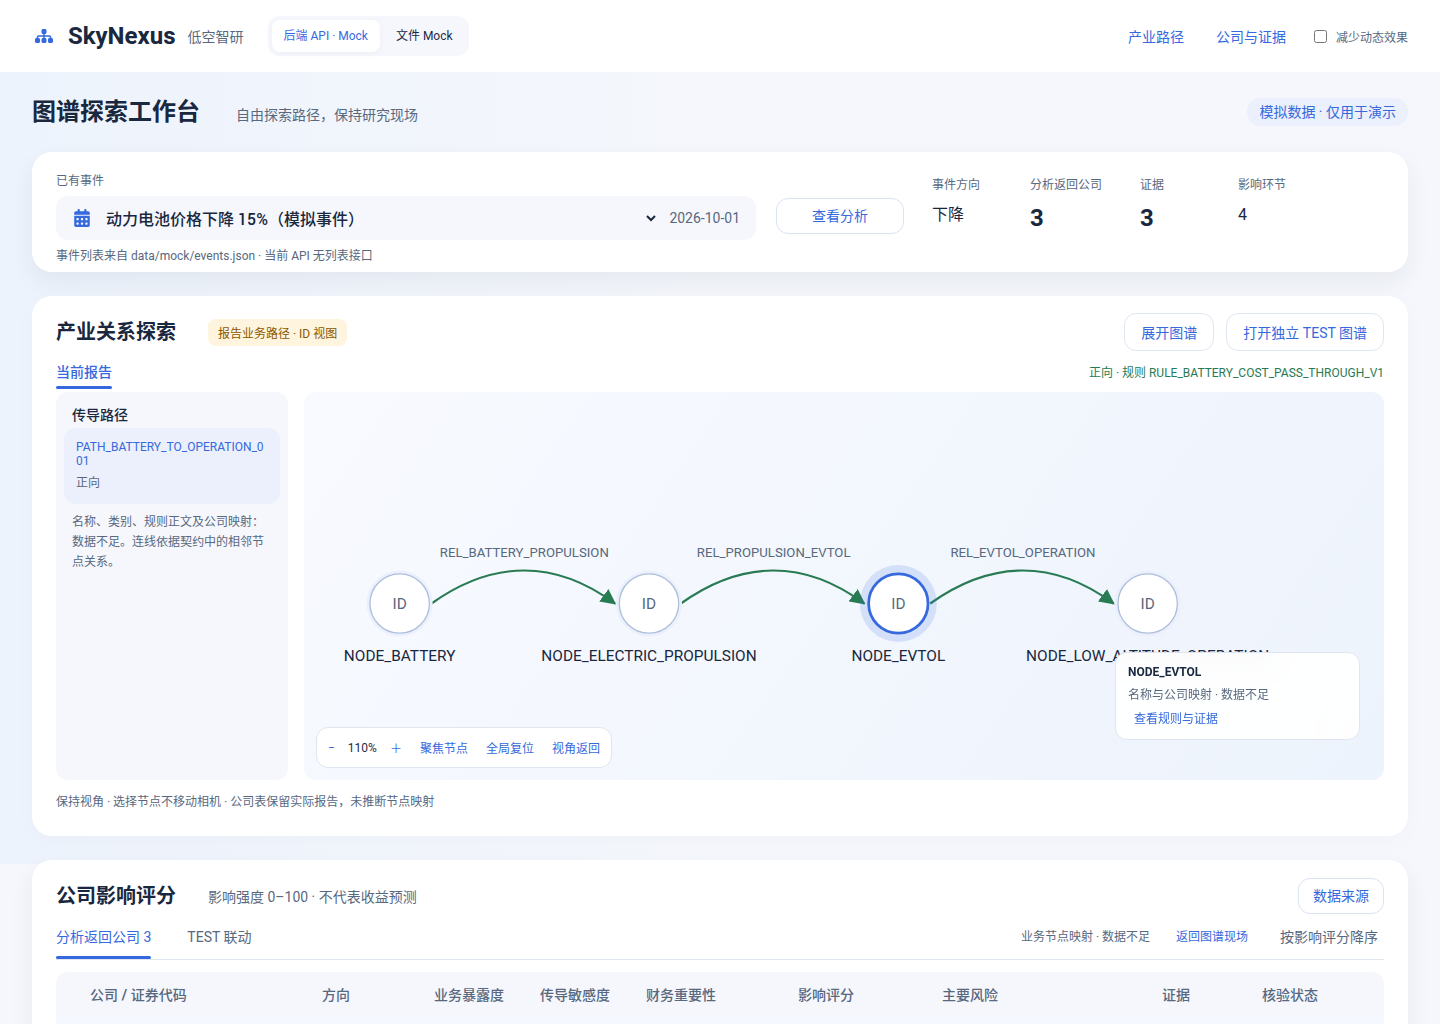
\includegraphics[width=0.90\linewidth,height=0.38\textheight,keepaspectratio]{assets/hongyulyu714-prog/fig-node-selection.png}
\PlanFigureCaption{图16-1}{路径节点选择与研究现场截图。研究者可以聚焦特定节点、阅读关联路径并保留当前视角；截图来源于\texttt{docs/screenshots/05-business-held.png}。这种交互将图谱阅读转化为对具体节点和关系的检验。}
\end{center}

传导分析区分四个概念：\textit{技术相邻}表示产品或工艺具有连接；\textit{业务关系}表示供应、采购、配套或运营服务等可描述关系；\textit{经济暴露}表示事件能够通过该关系影响成本、收入、资产或风险；\textit{证券主体关联}表示某一上市公司能够被明确映射到该业务环节。四层关系依次汇合为公司研究输入，链条、产品和主体证据共同支撑产业传导解释。

\begin{center}\small 表16-1\quad 图谱传导分析的审阅框架\par\vspace{1mm}
\begin{tabularx}{\linewidth}{p{0.18\linewidth}p{0.28\linewidth}X}
\toprule
分析层次 & 研究判断 & 可复核字段或材料\\
\midrule
事件--节点层 & 事件首先改变哪个产业对象，影响方向为何？ & \texttt{event\_id}、受影响\texttt{node\_id}、日期、方向与来源。\\
节点--关系层 & 哪些相邻节点能够构成有向传导路径？ & 有序节点ID、\texttt{relation\_ids}、关系类型、方向和路径长度检查。\\
关系--规则层 & 关系在哪些条件下适用，是否有例外或缺失信息？ & 规则ID、适用条件、规则来源、核验状态与数据不足提示。\\
路径--公司层 & 哪些证券主体确实处于路径相关的产品或业务环节？ & 证券代码、公司角色、公司--产品--节点映射与公司证据。\\
公司--财务层 & 事件通过何种成本、收入或风险变量影响研究对象？ & 暴露度、敏感度、财务重要性、影响方向、影响分与财务数据口径。\\
\bottomrule
\end{tabularx}\end{center}

独立图谱数据包现有35个节点、50条关系、25项公司映射和10条事件规则\cite{lhy-graph}。这些资产为后续统一查询提供了结构基础；当前Mock主链用业务ID路径验证接口、前端和运行记录，图谱资产将以同一契约完成接入。通过把资产规模、接入状态和报告实际消费的数据分别标记，项目能够在保持研究叙事连贯的同时，清晰呈现每一项传导结论的证据阶段。


% ===== merged source: pages/p17.tex =====
% !TEX root = ../main.tex
\subsection*{4.4 证据检索}\label{page:17}
\noindent\textbf{证据检索模块以可定位事实集合为起点，再组织可读的研究表达。}低空智研将事件ID、时间、地区、来源等级、证券代码和核验状态作为检索与表达的约束条件：证据先被筛选和定位，路径与公司再引用其\texttt{evidence\_ids}，报告语言据此概括事实、关系与公司影响\cite{lhy-evidence,lhy-contracts}。

证据最小单元由来源标题、发布日期、URL、原文定位、可引用短摘录、事件ID、显式证券代码、可信度与核验状态组成。研究者可以在界面中确认具体哪一句材料支持哪个事实，并将事件事实、公司主体和路径关系分别绑定到相应依据，形成颗粒度清晰的研究证据链。

\begin{center}\small 表17-1\quad 从检索条件到报告表述的证据约束\par\vspace{1mm}
\begin{tabularx}{\linewidth}{p{0.22\linewidth}p{0.30\linewidth}X}
\toprule
约束条件 & 在检索与绑定中的作用 & 对报告表述的限制\\
\midrule
事件ID与时间范围 & 将材料组织于同一研究对象及其有效时间语境 & 同一事件内的证据片段形成连续、可定位的事实序列。\\
地区与产业对象 & 区分适用市场、节点和业务范围 & 结论准确说明材料覆盖的对象与产业层级。\\
来源与定位 & 保留标题、URL、日期、短摘录和原文位置 & 读者可返回原文核对，并迅速定位支持性材料。\\
证券代码与公司映射 & 识别证据明确支持的上市主体 & 显式主体关联将公司研究建立在可审阅的证券实体基础上。\\
可信度与核验状态 & 区分线索、可复核材料、Mock记录和待核验记录 & 报告语言与状态一致；待核线索保留为研究任务，不升级为确定性陈述。\\
\bottomrule
\end{tabularx}\end{center}

仓库已形成30条事件、31条证据片段及30道评测题的独立证据资产，可作为后续检索、问答与人工复核的基准\cite{lhy-evidence}。该资产与当前\texttt{mock-v1}报告数据分开管理，接入时将以事件ID、证据ID和核验状态完成映射。这样的设计使大模型在未来能够承担候选事实提取、检索排序和受约束的报告组织任务，同时让事实边界、来源归属和引用完整性始终由可检查数据结构控制。

\noindent\textbf{由证据约束的报告生成，使每一句重要判断拥有明确的研究位置。}研究者获得一条能够从事件、路径和公司回到原始依据的连续解释；评审者也能够按证据、规则和计算逐层检查系统的事实基础。


% ===== merged source: pages/p18.tex =====
% !TEX root = ../main.tex
\subsection*{4.5 总控编排}\label{page:18}
\noindent\textbf{总控Agent以编排和核验将多源研究输出汇聚为一份统一报告。}一次分析从创建\texttt{run\_id}开始：总控根据请求选择已登记的数据版本，读取五类结构化输入，检查字段、引用和路径结构，复算影响强度，生成带报告ID、时间和状态的结果，并将处理结果写入运行记录。这个过程把事件、图谱、公司、财务和证据从并列文件组织为具有内部一致性的研究报告\cite{lhy-orchestrator,lhy-architecture}。

\begin{center}\small 表18-1\quad 单次编排运行的步骤、检查对象与研究意义\par\vspace{1mm}
\begin{tabularx}{\linewidth}{p{0.16\linewidth}p{0.32\linewidth}X}
\toprule
运行步骤 & 主要检查对象 & 形成的研究保障\\
\midrule
创建运行记录 & 请求事件、数据版本、开始时间与调用状态 & 每份报告均可识别其生成条件，并形成完整处理轨迹。\\
选择数据版本 & 数据源注册表和五类输入目录 & 同一分析中的事件、路径、评分和证据保持版本一致。\\
验证事件与路径 & 事件存在性、节点数量、关系数量、关系连通性 & 保证分析围绕有效事件，并使每一条路径保持可读、可检查的结构。\\
验证公司与评分 & 证券代码、方向、分数范围、公式结果与风险标记 & 使公司条目拥有明确主体和可复算的影响强度。\\
绑定证据与结论 & 路径/结论引用的证据ID及公司显式关联 & 报告中的关键主张获得可回溯的证据入口。\\
写入结果状态 & 完成时间、报告ID或错误文本 & 支持前端反馈、问题定位、回归测试与同事件的版本对照。\\
\bottomrule
\end{tabularx}\end{center}

总控将确定性规则置于跨模块接口处。数据版本经注册后参与分析，路径关系数与节点数保持匹配，影响分通过公式复算，报告中的证据引用与事件集合一一对应。这些规则将研究过程中的隐含假设显式化，使团队能够以测试、运行记录和数据版本共同维护同一条研究链\cite{lhy-contracts,lhy-orchestrator}。

未来多智能体协作将以此为基础展开：事件Agent、图谱Agent、财务Agent和证据Agent并行产生候选结果，候选结果归一到同一契约后进入版本、结构、计算和证据检查。智能体的信息抽取与检索效率由此与最终研究产物的可审阅、可复跑和可定位性质统一起来。

从智能体协作视角看，低空智研定义了一种面向金融研究的“强约束协同”范式。每个Agent围绕自身专业对象工作：事件Agent关注事实、时间与影响方向，图谱Agent关注传导链条与规则，财务Agent关注参数和影响强度，证据Agent关注来源与定位；总控Agent将这些输出编排为报告。分工提升了研究深度，统一契约保证了不同专业判断能够在同一事件下汇合。


% ===== merged source: pages/p19.tex =====
% !TEX root = ../main.tex
\subsection*{4.6 一致性检查}\label{page:19}
\noindent\textbf{系统可靠性建立在贯穿输入、关系、计算和引用的可执行校验之上。}低空智研将跨模块约束写为规则，覆盖数据版本、事件、路径结构、证券主体、影响分、证据引用和运行状态。每次分析均将这些结构条件写入运行记录，使研究质量控制嵌入报告生成过程，并可由同一规则持续复核\cite{lhy-contracts,lhy-orchestrator}。

\begin{center}\small 表19-1\quad 已实现质量闸门及其对研究报告的作用\par\vspace{1mm}
\begin{tabularx}{\linewidth}{p{0.23\linewidth}p{0.29\linewidth}X}
\toprule
质量闸门 & 核验对象 & 对报告和运行记录的作用\\
\midrule
版本与事件检查 & 事件、数据版本、路径及其对应输入的匹配关系 & 为每次运行建立完整的数据来源、输入范围和处理状态记录。\\
路径结构检查 & 节点数量、关系数量和逐段连接关系 & 使每条路径保持连通、可读并可逐段审阅的传导结构。\\
主体与证据检查 & 证券代码、公司显式证据关联和引用ID & 使公司、证据与结论形成清晰、可定位的主体关联。\\
评分复算检查 & 影响分与$E\times S\times F/10000$的计算一致性 & 将公司代码、参数、公式和计算结果共同保留为可复算解释。\\
结论引用检查 & 路径或结论与当前事件证据集合的对应关系 & 使研究结论与事件、路径、公司和证据保持一一对应。\\
\bottomrule
\end{tabularx}\end{center}

这些检查构成项目工程可靠性的直接证据：同一接口、数据版本和公式在既定条件下持续验证。事件级评测围绕路径边正确性、证据事实支持、公司主体匹配、影响方向解释与研究效率展开；工程验证与研究评测共同构成系统性能的证据体系。

\noindent\textbf{因此，本项目将可靠性理解为一条由数据治理、结构校验、计算复核、证据定位和任务评测共同构成的证据链。}这一结构适合低空产业这种跨技术、跨制造、跨运营的复杂研究场景，并为数据更新、规则扩展和模型接入提供共同的质量坐标。研究者阅读报告时看到的路径、公司和分数，均对应同一套输入、规则和引用关系；研发人员更新任一模块时，也可通过运行记录定位其对研究结论的实际影响。


% ===== merged source: pages/p20.tex =====
% !TEX root = ../main.tex
\subsection*{4.7 工程实现}\label{page:20}
\noindent\textbf{项目以可复现的本地研究演示为工程起点，前后端通过稳定HTTP接口解耦。}后端使用Python、FastAPI、Pydantic与Uvicorn，承担事件分析、总控编排、契约校验与运行记录；前端使用React、TypeScript与Vite，承担研究发起、路径阅读、公司比较与证据回溯。默认开发环境中，后端服务监听本地\texttt{8000}端口，前端开发服务监听\texttt{5173}端口，并将\texttt{/api}和\texttt{/health}请求代理给后端\cite{lhy-repository,lhy-frontend}。

工程解耦让研究界面与数据资产能够同步演进。前端以结构化报告和状态字段组织阅读；后端以注册数据版本读取输入；图谱、证据、财务数据和模型输出在契约内持续升级。接口兼容性由测试和版本门禁维护，使研究界面、报告阅读与数据治理形成稳定协同。

\begin{center}
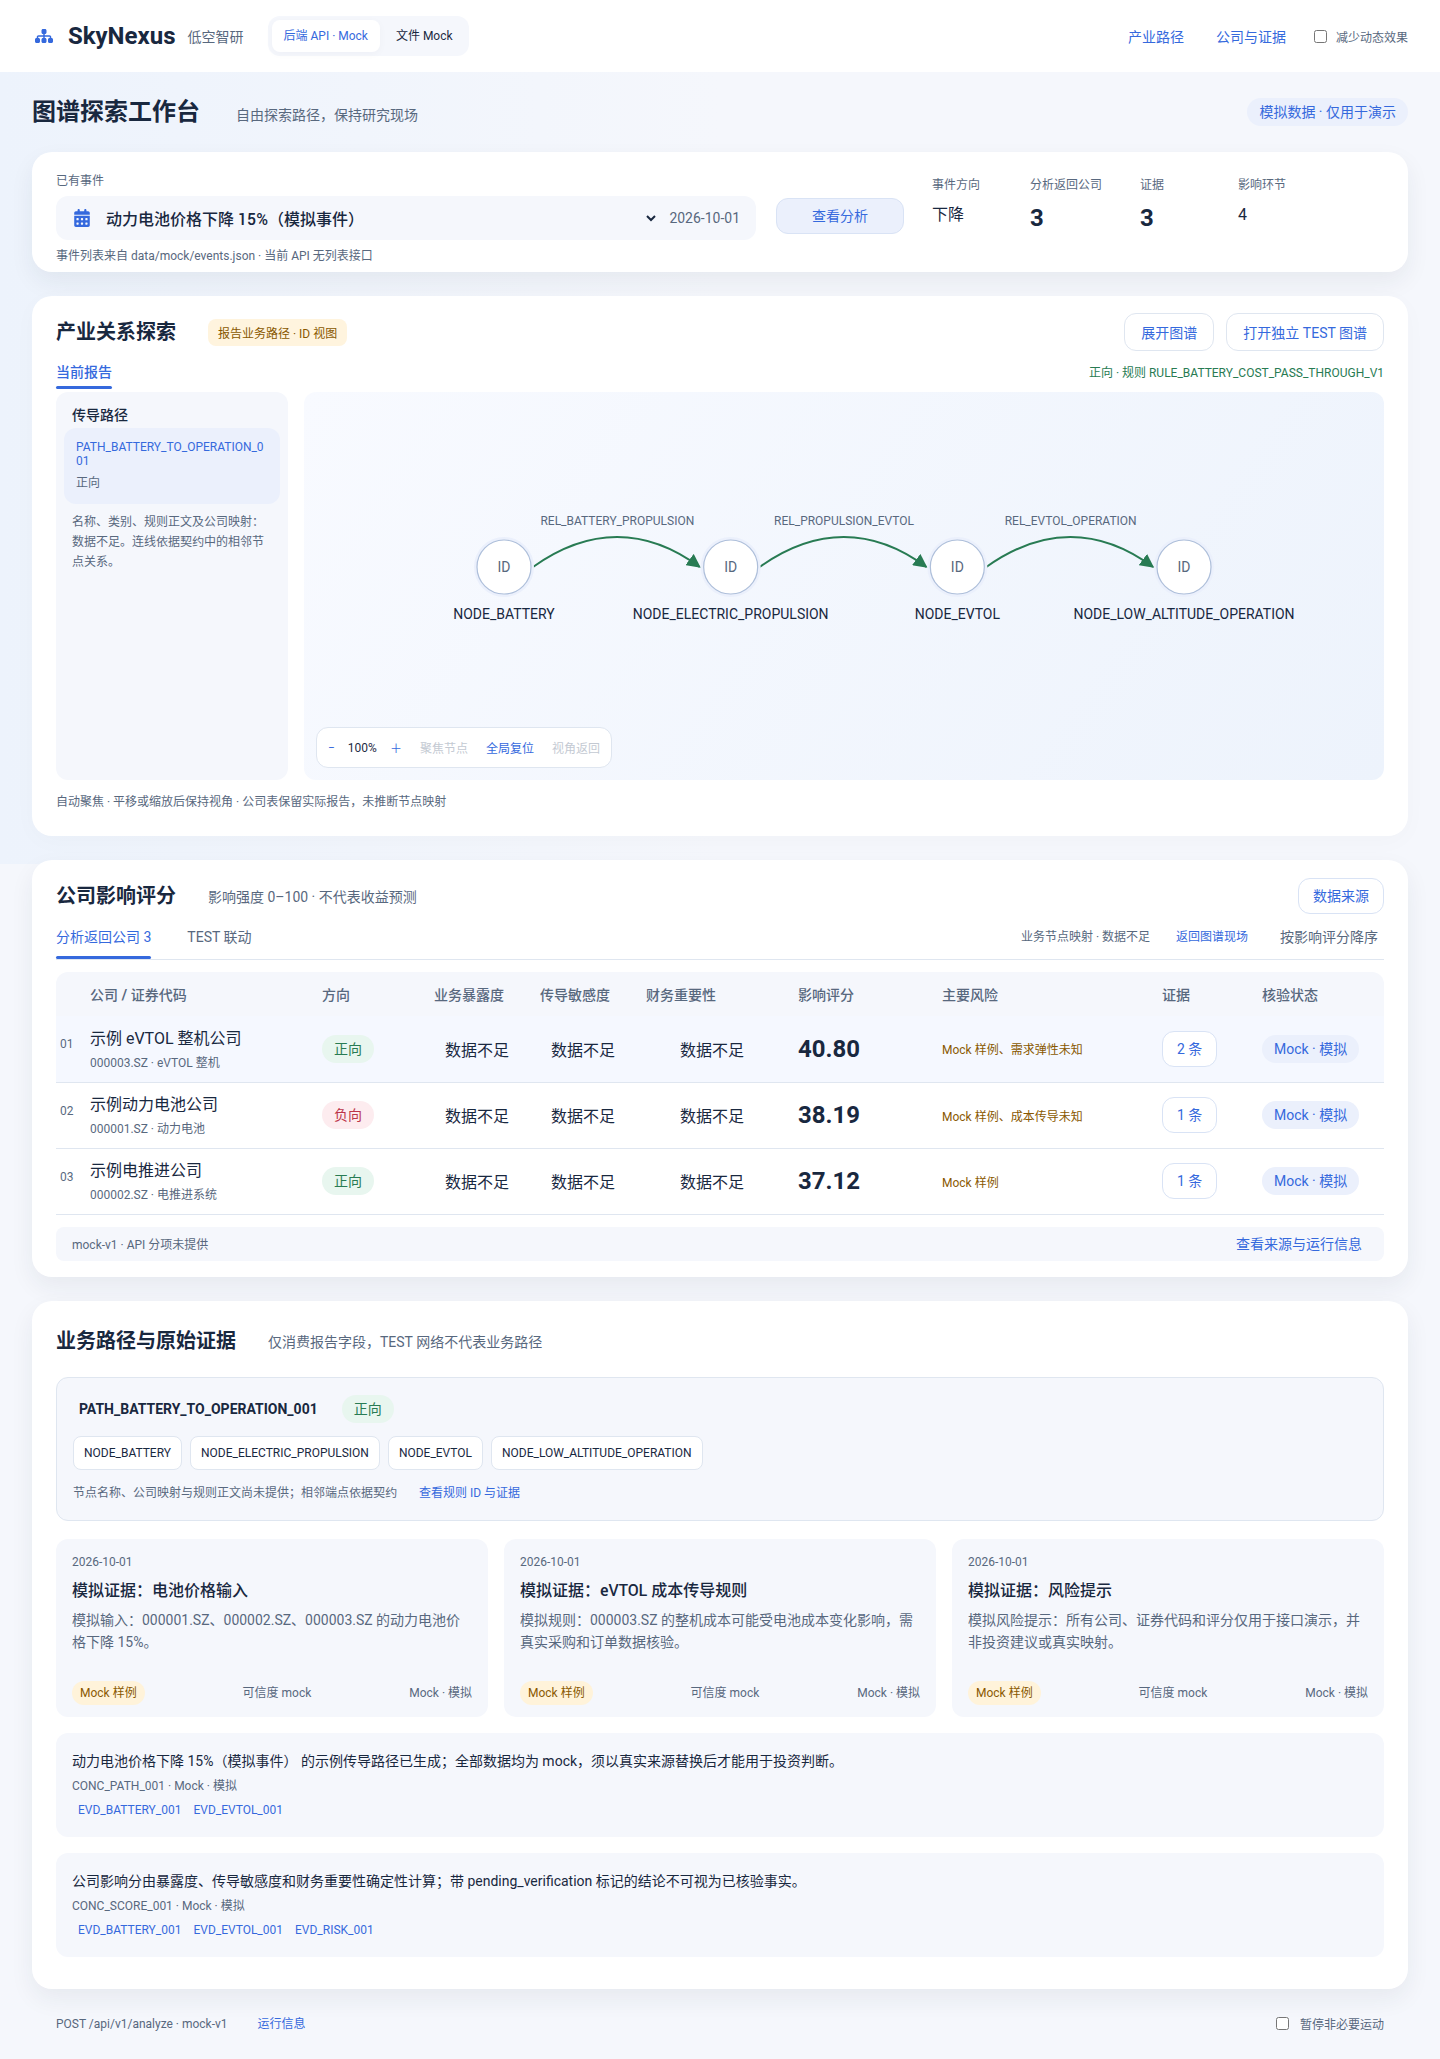
\includegraphics[width=0.93\linewidth,height=0.40\textheight,keepaspectratio]{assets/hongyulyu714-prog/fig-full-report.png}
\PlanFigureCaption{图20-1}{完整研究报告界面截图。图中展示工作台在一次分析完成后组织事件、路径、公司和证据对象的方式；截图来源于\texttt{docs/screenshots/04-business-full.png}。该页面呈现的是\texttt{mock-v1}下的可复现研究流程。}
\end{center}

\begin{center}\small 表20-1\quad 工程层、当前配置与复现要求\par\vspace{1mm}
\begin{tabularx}{\linewidth}{p{0.18\linewidth}p{0.29\linewidth}X}
\toprule
工程层 & 实现配置 & 复现与演进要求\\
\midrule
分析服务 & FastAPI接口、Pydantic数据模型、总控与本地运行记录 & 每次分析保留事件ID、版本、运行状态与报告ID，形成可追溯的处理记录。\\
研究前端 & React/TypeScript工作台、路径交互、公司卡片与证据抽屉 & 以API返回的状态驱动展示；API模式与文件Mock模式在界面中明确区分。\\
数据目录 & 默认\texttt{mock-v1}五类JSON与独立图谱、证据、评分资产 & 数据接入同步登记来源、口径、版本、权限和核验状态，并遵循项目的数据治理与交付规范。\\
自动化验证 & 前端单测、浏览器场景、后端测试、类型检查、Lint、构建和CI & 验证记录与具体提交、环境和命令对应，用于保障工程链路的可重复执行。\\
产品化环境 & 本地演示与部署演进路径 & 采用同源反向代理、受控服务进程、访问审计和版本化数据源承接，并完成权限与性能专项验收。\\
\bottomrule
\end{tabularx}\end{center}

仓库记录的验证包括31项前端单元测试、20个Linux Chrome端到端场景和37项后端测试，并已完成类型检查、Lint、构建及三平台CI验证\cite{lhy-repository,lhy-frontend}。这些验证记录为产业路径、证据和公司研究的事件级评测提供稳定基础；固定任务、人工复核和对照实验将持续积累金融研究效果证据。工程可复现性由此成为研究可验证性的基础设施。


% ===== merged source: pages/p21.tex =====
% !TEX root = ../main.tex
\clearpage
\section{数据体系与金融评分}
\subsection*{数据来源与版本管理}\label{page:21}
\ifdraftversion{\noindent\small\color{gray}写作页位 21\quad 负责人 武桐宇\par}\fi
\WritingGuide{说明公开证据、图谱和授权财务的来源与更新。}{数据来源与更新表。}{时间、单位、授权及数据状态可追溯。}
\NeedEvidence{替换本页写作指引，补入正文、真实材料与可定位出处。}
\FigureSlot{数据来源与版本管理所需图表}{数据来源与更新表。}

% 按“一句话结论—证据—解释—适用条件”组织本页正文。


% ===== merged source: pages/p22.tex =====
% !TEX root = ../main.tex
\PlanPage{产业图谱与公司映射}{武桐宇}{22}
\WritingGuide{解释节点、关系、公司产品与映射方法。}{实际资产清单及映射实例。}{产品匹配代理不得冒充相关业务收入占比。}
\NeedEvidence{替换本页写作指引，补入正文、真实材料与可定位出处。}
\FigureSlot{产业图谱与公司映射所需图表}{实际资产清单及映射实例。}

% 按“一句话结论—证据—解释—适用条件”组织本页正文。


% ===== merged source: pages/p23.tex =====
% !TEX root = ../main.tex
\PlanPage{财务字段与清洗}{武桐宇}{23}
\WritingGuide{交代合并报表、单季、同日估值和异常处理。}{字段字典和处理例子。}{不能把累计季度数直接当单季数。}
\NeedEvidence{替换本页写作指引，补入正文、真实材料与可定位出处。}
\FigureSlot{财务字段与清洗所需图表}{字段字典和处理例子。}

% 按“一句话结论—证据—解释—适用条件”组织本页正文。


% ===== merged source: pages/p24.tex =====
% !TEX root = ../main.tex
\PlanPage{公司影响评分}{武桐宇}{24}
\WritingGuide{解释三个分项、公式、参数和方向。}{手算例子、符号和参数依据。}{公式为E乘S乘F除以10000；财务分项是放大程度代理。}
\begin{equation}
I=\frac{E\times S\times F}{10000},\qquad E,S,F,I\in[0,100].
\end{equation}
其中，$E$ 为业务暴露度，$S$ 为事件传导敏感度，$F$ 为财务重要性分项，$I$ 为影响强度。方向单独记录。该式对应仓库当前评分代码，参数与适用条件由作者根据所用版本补齐。
\SourceNote{\texttt{backend/scoring.py}；\texttt{docs/SCORING\_METHOD.md}，取材时记录提交版本。}

% 按“一句话结论—证据—解释—适用条件”组织本页正文。


% ===== merged source: pages/p25.tex =====
% !TEX root = ../main.tex
\PlanPage{数据质量与评分验证}{武桐宇}{25}
\WritingGuide{展示来源抽查、公式复算和敏感性验证。}{抽查记录与参数变化结果。}{模拟财务与正式授权数据分别标注。}
\NeedEvidence{替换本页写作指引，补入正文、真实材料与可定位出处。}
\FigureSlot{数据质量与评分验证所需图表}{抽查记录与参数变化结果。}

% 按“一句话结论—证据—解释—适用条件”组织本页正文。


% ===== merged source: pages/p26.tex =====
% !TEX root = ../main.tex
\clearpage
\section{应用案例与效果验证}
\subsection*{6.1 评测框架}\label{page:26}
\noindent\textbf{金融人工智能系统的评价由工程可运行性、产业路径正确性、证据可追溯性、公司研究队列质量和研究效率共同构成。}五类任务分别回答系统运行、传导解释、结论来源、主体与分数审阅、研究效率等关键问题。所有任务在执行前冻结代码提交、数据版本、事件清单、评分公式版本、任务说明与复核规则，使不同方法在共同条件下获得可比较的结果。

\begin{center}\small 表26-1\quad 面向事件驱动投研的分层评测协议\par\vspace{1mm}
\begin{tabularx}{\linewidth}{p{0.18\linewidth}p{0.34\linewidth}X}
\toprule
评测层次 & 任务、对照与主要指标 & 需要保留的原始记录\\
\midrule
工程闭环 & 固定事件的健康检查、分析请求、报告字段与前端呈现；记录接口成功率与异常路径覆盖 & 提交版本、环境、请求、响应、\texttt{run\_id}、错误信息和截图。\\
产业路径 & 对固定事件题逐边判断节点、方向、关系和适用条件；对照为依据原始材料绘制的人工路径 & 路径边精确率、召回率、整路径一致率、每条边的证据与复核意见。\\
证据链 & 抽取每条结论的\texttt{evidence\_ids}，核对URL、日期、摘录、主体和支持范围 & 可定位率、事实支持率、错误引用类型、证据状态与复核人意见。\\
公司队列与评分 & 以已核验主体映射和授权财务数据为对照，分别检查公司、方向和分数 & 主体匹配率、方向一致率、分数复算一致率、参数版本与人工裁决记录。\\
研究效率与可用性 & 在同一任务脚本下比较人工检索、文档检索和完整工作流 & 完成时间、中断次数、返工次数、引用完整性、用户操作记录与开放反馈。\\
\bottomrule
\end{tabularx}\end{center}

评测采用“双人独立复核—记录分歧—依据原始材料裁决”的过程。路径、公司和证据任务的判定不依赖系统自己生成的解释，而由复核者按照预先定义的判定单元进行标注：路径以边为单位，证据以可定位事实为单位，公司以证券主体为单位，评分以输入参数和公式为单位。若出现分歧，保留原始判定和裁决依据，使后续迭代可以区分是数据问题、规则问题还是界面表达问题。

仓库已有30条事件、31条证据片段和30道评测题，构成任务集的结构化起点\cite{lhy-evidence}。\texttt{mock-v1}主链已经提供端到端运行条件；图谱、证据和评分资产进入统一契约后，项目将按本页协议系统报告路径、证据、公司与效率指标。该方案以多层指标呈现研究结论的事实基础、传导逻辑和应用价值。


% ===== merged source: pages/p27.tex =====
% !TEX root = ../main.tex
\subsection*{6.2 流程演示}\label{page:27}
\noindent\textbf{完整流程演示以固定事件和固定数据版本呈现一份事件研究报告如何形成。}演示使用\texttt{EVT\_BATTERY\_PRICE\_DOWN\_001}与\texttt{mock-v1}：研究者在“后端API·Mock”模式下选择“动力电池价格下降15\%”，发起一次分析请求，获得包含运行信息的结构化报告。该报告包含4个路径环节、3家分析返回公司和3条证据记录，完整呈现事件、路径、公司与证据如何汇入同一研究现场\cite{lhy-frontend,lhy-architecture}。

\begin{center}
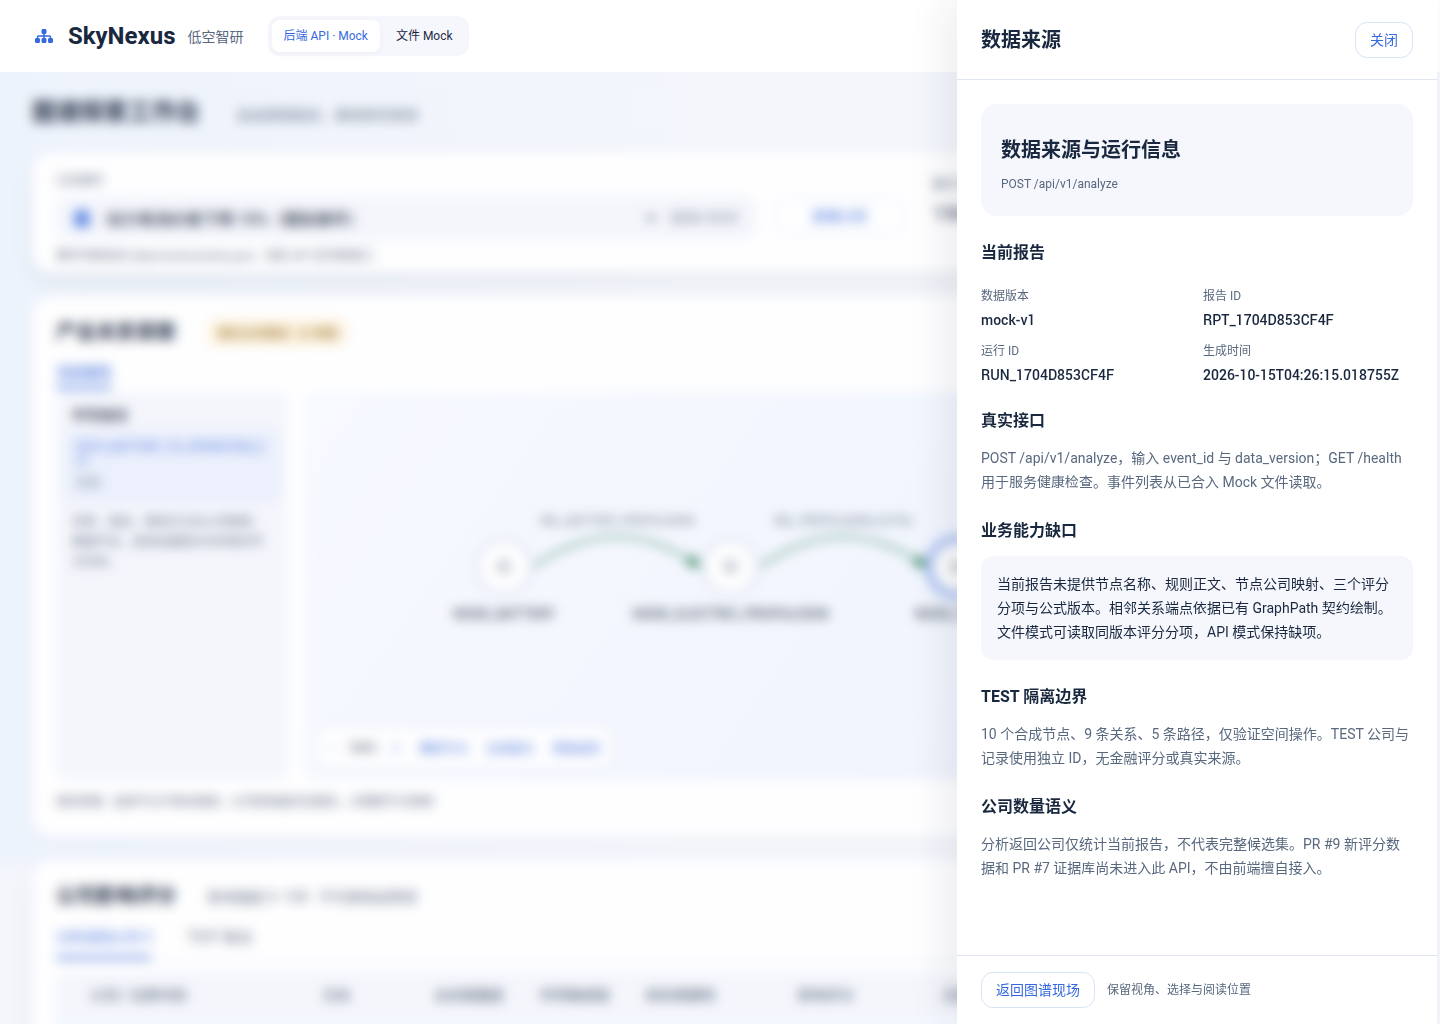
\includegraphics[width=0.92\linewidth,height=0.41\textheight,keepaspectratio]{assets/hongyulyu714-prog/fig-report-source.png}
\PlanFigureCaption{图27-1}{报告来源与运行信息界面。页面展示数据版本、运行信息和来源入口；截图来源于\texttt{docs/screenshots/10-sources.png}。这些字段使一份可视化报告同时保留可追溯的生成条件。}
\end{center}

\begin{center}\small 表27-1\quad 三分钟演示的研究阅读顺序与检查要点\par\vspace{1mm}
\begin{tabularx}{\linewidth}{p{0.15\linewidth}p{0.35\linewidth}X}
\toprule
时段 & 演示动作 & 评审者可直接检查的研究对象\\
\midrule
0:00--0:30 & 选择事件，确认“后端API·Mock”模式与数据版本，发起分析 & 事件名称、\texttt{event\_id}、\texttt{mock-v1}、\texttt{run\_id}、生成时间与状态。\\
0:30--1:10 & 阅读业务ID路径，切换节点、路径与视角 & 每条连线的相邻节点、关系ID、路径方向、规则和证据阅读入口。\\
1:10--1:45 & 打开公司影响列表及单家公司详情 & 证券主体、产业角色、影响方向、影响强度、风险标记、评分构成与证据ID。\\
1:45--2:20 & 打开电池价格输入的证据，检查标题、日期、摘录与来源入口 & Mock状态、可信度、核验标签与该证据支持的事实范围。\\
2:20--3:00 & 打开报告来源与运行信息，回到研究现场复核 & 报告数据版本、运行记录、来源信息、路径与证据之间的对应关系。\\
\bottomrule
\end{tabularx}\end{center}

该演示以公司卡片、产业路径、事件规则、证据抽屉与运行记录构成连续审阅路线。研究者可从公司卡片进入影响参数，再回到产业路径和证据抽屉；评审者可从报告ID回到运行记录，复核本次结论所消费的数据版本。示例中eVTOL公司显示的40.80为Mock影响强度，观众可以据此检查参数、方向、报告字段和证据绑定方式。事件、路径、公司、证据和运行状态因而被组织为一份可连续阅读、可逐层核对的研究记录。


% ===== merged source: pages/p28.tex =====
% !TEX root = ../main.tex
\PlanPage{政策事件案例}{武桐宇}{28}
\WritingGuide{核对政策地区、对象、时效及影响路径。}{原始政策、路径、公司研究对象。}{政策部署不等于订单、收入或已拨款。}
\NeedEvidence{替换本页写作指引，补入正文、真实材料与可定位出处。}
\FigureSlot{政策事件案例所需图表}{原始政策、路径、公司研究对象。}

% 按“一句话结论—证据—解释—适用条件”组织本页正文。


% ===== merged source: pages/p29.tex =====
% !TEX root = ../main.tex
\PlanPage{原材料价格案例}{武桐宇}{29}
\WritingGuide{解释上下游方向、成本传导条件与公司暴露。}{同口径价格资料和条件分析。}{行业材料价格不能直接替代航空级报价。}
\NeedEvidence{替换本页写作指引，补入正文、真实材料与可定位出处。}
\FigureSlot{原材料价格案例所需图表}{同口径价格资料和条件分析。}

% 按“一句话结论—证据—解释—适用条件”组织本页正文。


% ===== merged source: pages/p30.tex =====
% !TEX root = ../main.tex
\PlanPage{适航或订单案例}{武桐宇}{30}
\WritingGuide{核对主体、产品、进展阶段与商业关系。}{原公告、路径和条件。}{TC、PC、OC及订单、计划、交付分别陈述。}
\NeedEvidence{替换本页写作指引，补入正文、真实材料与可定位出处。}
\FigureSlot{适航或订单案例所需图表}{原公告、路径和条件。}

% 按“一句话结论—证据—解释—适用条件”组织本页正文。


% ===== merged source: pages/p31.tex =====
% !TEX root = ../main.tex
\subsection*{6.3 对照实验}\label{page:31}
\noindent\textbf{完整工作流的价值由同一任务、同一材料和同一复核标准构成的对照体系检验。}项目将人工原始材料检索、通用摘要/问答、文档检索、结构化完整流程及两个关键模块变体纳入预注册对照。比较聚焦路径准确性、证据可定位性、主体一致性和任务完成效率；每项指标均对应明确的判定对象、复核规则和原始记录。

\begin{center}\small 表31-1\quad 对照与消融设置的研究问题设计\par\vspace{1mm}
\begin{tabularx}{\linewidth}{p{0.20\linewidth}p{0.33\linewidth}X}
\toprule
设置 & 研究能力配置 & 主要回答的问题\\
\midrule
人工原始材料检索 & 研究者自行阅读公开材料、形成路径和公司清单 & 建立人工基准，记录完成同一任务的时间与人工整理成本。\\
通用摘要/问答 & 输入相同问题，输出阅读摘要与问答结果 & 考察摘要式阅读在路径、证券主体和证据定位维度上的表现。\\
文档检索流程 & 返回相关片段和链接，形成检索结果集 & 考察检索结果如何支持产业传导阅读与公司解释。\\
完整工作流 & 事件、路径、公司、评分和证据经总控组合为报告 & 跨模块结构化编排是否提升路径、引用和队列的一致性？\\
路径约束变体 & 保留证据和评分，改变路径与规则的呈现配置 & 产业路径如何影响研究者解释传导机制和复核公司关联。\\
证据约束变体 & 保留路径与排序，改变\texttt{evidence\_ids}绑定配置 & 证据绑定如何影响结论可定位率与事实支持率。\\
\bottomrule
\end{tabularx}\end{center}

所有设置使用同一事件题、相同截止日期的材料、相同公司范围和相同答题模板。至少两名复核者在不知晓方法来源的条件下，对事件事实、路径边、公司主体与证据定位分别判定；项目记录路径边精确率与召回率、证据可定位率、事实支持率、主体匹配率、评分复算一致率及完成时间中位数。对于路径解释类任务，除数值指标外，复核表还记录错误发生在事件识别、关系方向、公司映射、财务解释还是证据引用层。

这一对照设计使不同模块承担明确的证据角色：图谱模块检验传导解释，证据模块检验引用完整性，评分模块检验计算可复现性，总控模块检验跨模块一致性。实验按预注册协议运行，现有契约测试、接口验证和运行记录构成工程基线；随着数据主链完成接入，固定任务集将持续沉淀面向事件级研究效果的可比较证据。


% ===== merged source: pages/p32.tex =====
% !TEX root = ../main.tex
\subsection*{6.4 验证设计}\label{page:32}
\noindent\textbf{可复现验证已经表明，系统工程主链具备稳定的接口、交互和状态处理能力；事件级研究评测将以这条主链为基础展开。}仓库在前端实现提交\texttt{86a440a}的验证记录中报告：31项前端单元测试、20个Linux Chrome端到端场景和37项后端测试通过，同时完成类型检查、Lint、生产构建与三平台CI。它们共同检验事件选择、服务联调、路径与节点交互、公司显示、证据抽屉、状态处理以及构建过程是否在规定环境下稳定执行\cite{lhy-repository,lhy-frontend}。

\begin{center}\small 表32-1\quad 已有系统验证及其在研究评价中的位置\par\vspace{1mm}
\begin{tabularx}{\linewidth}{p{0.20\linewidth}p{0.22\linewidth}X}
\toprule
验证记录 & 已报告结果 & 对后续研究评测提供的基础\\
\midrule
前端单元测试 & 31项通过 & 保证组件、数据适配和关键交互逻辑在既定断言下可重复执行。\\
浏览器端到端场景 & Linux Chrome 20个通过 & 验证事件选择、分析请求、路径阅读、公司页面、证据抽屉与研究现场恢复能够贯通。\\
后端测试 & 37项通过 & 覆盖事件、版本、路径、评分与证据引用的核心正常/异常条件，为数据接入提供回归门槛。\\
类型检查、Lint与构建 & 已完成 & 保障前端工程在固定依赖与构建链中保持一致，可作为演示版本冻结的技术依据。\\
三平台CI & 已记录安装与构建验证 & 说明工程交付不依赖单一开发设备，为比赛展示和后续协作提供复现条件。\\
\bottomrule
\end{tabularx}\end{center}

研究使用验证沿用同样的可复现原则。试用者按照统一任务脚本完成一次事件研究，系统记录版本、任务、开始与完成时间、打开过的证据、来源定位情况、人工修正环节以及开放意见。反馈记录与具体任务、界面和版本绑定，使产品团队能够依据可定位问题迭代路径规则、证据呈现和公司比较，并持续积累任务层面的研究质量证据。

\noindent\textbf{工程验证与研究验证在本项目中形成递进关系。}前者确保同一数据和方法在多次运行中产生可比较的报告，后者检验报告是否帮助研究者更准确、更高效地完成事件驱动分析。以固定任务、原始材料、双人复核和版本化记录连接这两类验证，项目能够持续积累面向金融人工智能赛题的可信证据。


% ===== merged source: pages/p33.tex =====
% !TEX root = ../main.tex
\clearpage
\section{创新点与竞争分析}
\subsection*{金融研究方法上的改进}\label{page:33}
\ifdraftversion{\noindent\small\color{gray}写作页位 33\quad 负责人 武桐宇\par}\fi
\WritingGuide{围绕具体研究任务解释方法贡献。}{设计、问题与验证依据的对应表。}{创新主张限制在证据支持的范围。}
\NeedEvidence{替换本页写作指引，补入正文、真实材料与可定位出处。}
\FigureSlot{金融研究方法上的改进所需图表}{设计、问题与验证依据的对应表。}

% 按“一句话结论—证据—解释—适用条件”组织本页正文。


% ===== merged source: pages/p34.tex =====
% !TEX root = ../main.tex
\PlanPage{同类工具与方法比较}{武桐宇}{34}
\WritingGuide{按同一任务比较终端、问答、检索和图谱。}{有日期、版本和来源的比较表。}{不编造竞品能力，不只选择弱基线。}
\NeedEvidence{替换本页写作指引，补入正文、真实材料与可定位出处。}
\FigureSlot{同类工具与方法比较所需图表}{有日期、版本和来源的比较表。}

% 按“一句话结论—证据—解释—适用条件”组织本页正文。


% ===== merged source: pages/p35.tex =====
% !TEX root = ../main.tex
\PlanPage{自研成果与持续积累}{武桐宇}{35}
\WritingGuide{列明数据、规则、评分、接口与交互的自研贡献。}{开源复用与自研边界清单。}{如实保留外部来源与许可说明。}
\NeedEvidence{替换本页写作指引，补入正文、真实材料与可定位出处。}
\FigureSlot{自研成果与持续积累所需图表}{开源复用与自研边界清单。}

% 按“一句话结论—证据—解释—适用条件”组织本页正文。


% ===== merged source: pages/p36.tex =====
% !TEX root = ../main.tex
\clearpage
\section{市场进入与商业模式}
\subsection*{首批用户与市场入口}\label{page:36}
\ifdraftversion{\noindent\small\color{gray}写作页位 36\quad 负责人 武桐宇\par}\fi
\WritingGuide{从可触达用户和实际任务确定试点入口。}{用户触达与需求依据。}{市场测算不用宏观产业规模代替产品市场。}
\NeedEvidence{替换本页写作指引，补入正文、真实材料与可定位出处。}
\FigureSlot{首批用户与市场入口所需图表}{用户触达与需求依据。}

% 按“一句话结论—证据—解释—适用条件”组织本页正文。


% ===== merged source: pages/p37.tex =====
% !TEX root = ../main.tex
\PlanPage{服务形式与定价验证}{武桐宇}{37}
\WritingGuide{比较工作台、订阅、接口和部署服务。}{交付物、收费对象和价格假设。}{报价、意愿与成交事实分别记录。}
\NeedEvidence{替换本页写作指引，补入正文、真实材料与可定位出处。}
\FigureSlot{服务形式与定价验证所需图表}{交付物、收费对象和价格假设。}

% 按“一句话结论—证据—解释—适用条件”组织本页正文。


% ===== merged source: pages/p38.tex =====
% !TEX root = ../main.tex
\PlanPage{试点与转化计划}{武桐宇}{38}
\WritingGuide{安排试用、反馈、迭代及付费验证。}{试点周期、验收和维护责任。}{没有合作协议不得写成已达成合作。}
\NeedEvidence{替换本页写作指引，补入正文、真实材料与可定位出处。}
\FigureSlot{试点与转化计划所需图表}{试点周期、验收和维护责任。}

% 按“一句话结论—证据—解释—适用条件”组织本页正文。


% ===== merged source: pages/p39.tex =====
% !TEX root = ../main.tex
\clearpage
\section{实施计划与成果管理}
\subsection*{8.1 集成计划}\label{page:39}
\noindent\textbf{项目下一阶段将既有研究资产汇入同一条可审阅主链。}总控、API、研究工作台和Mock端到端流程已经构成可运行骨架；产业图谱、公司映射、证据库、评测题和评分样例提供了可扩展的独立资产。实施工作围绕统一事件和数据版本展开：一个事件同时解析为路径、公司、评分和证据，每项输出均由报告ID和运行记录串联，形成从数据资产到研究报告的连续交付。

\begin{center}\small 表39-1\quad 当前资产、集成目标与验收证据\par\vspace{1mm}
\begin{tabularx}{\linewidth}{p{0.20\linewidth}p{0.28\linewidth}X}
\toprule
资产 & 进入主链的具体目标 & 验收时应形成的证据\\
\midrule
统一契约、总控与API & 为图谱、证据和评分数据登记版本，保持报告字段兼容 & 端到端请求、报告JSON、运行记录、异常路径测试与接口变更说明。\\
React研究工作台 & 使不同数据源下的状态、来源和核验语义保持一致 & 固定提交的截图、浏览器场景、交互测试和字段显示对照。\\
产业图谱与公司映射 & 将节点、关系、规则和公司映射按事件调用并逐项检查 & 路径边来源、规则条件、证券主体与公司--产品--节点映射复核表。\\
事件证据与评测题 & 以事件ID接入检索与报告，保证证据可定位 & 证据账本、链接与摘录核验、题目外键检查和人工复核记录。\\
评分样例与公式 & 以明确口径接入财务变量并复算每条影响强度 & 公司代码、报告期、单位、参数、公式版本与复算结果。\\
研究效果评测 & 依据页26--32的固定协议运行对照与使用任务 & 冻结任务集、基线输出、指标、样本、分歧记录与原始结果文件。\\
\bottomrule
\end{tabularx}\end{center}

实施过程中，每项资产先完成来源、版本、字段、责任人和核验状态登记，再以固定事件进入报告联调，随后进入任务评测与演示版本。该顺序将数据、映射、接口、公式与前端表达纳入同一条可定位链路。项目由此形成“资产登记—契约接入—事件联调—任务评测—演示固化”的闭环，使研发进度由报告、记录、复核表和演示结果等可检查产物衡量。

\noindent\textbf{清晰的状态语言是成果管理的一部分。}“已实现”对应可运行代码或接口，“已测试”对应明确条件下的验证记录，“Mock”对应演示和复现数据，“已交付、接入中”对应具有独立结构和来源说明的数据包。通过这一标记体系，比赛材料将工程基础、数据资产和实施路线置于同一证据框架中，使每一项陈述均可回到仓库中的代码、数据或验证记录\cite{lhy-repository,lhy-architecture}。

统一主链还将改变低空经济研究资产的使用方式。图谱不再只是静态产业链图，证据不再只是附件目录，评分也不再是脱离事件背景的单行数值；三者围绕相同的事件ID、公司实体和报告版本共同工作。研究者据此能够在一份报告内完成事件影响的初步筛选、传导机制的逐边阅读、公司队列的比较和关键事实的来源回查，为投研团队建立可积累、可复用的低空专题研究底座。


% ===== merged source: pages/p40.tex =====
% !TEX root = ../main.tex
\subsection*{8.2 实施路线}\label{page:40}
\noindent\textbf{实施路线由可复核产物和研究问题共同推进。}每一阶段均对应一个明确问题：研究材料是否一致、数据能否进入同一主链、产业传导与证据如何接受评测、研究者如何在受控任务下使用系统，以及系统如何形成更大范围试用所需的治理条件。阶段转换由验收材料触发，使数据和模型的扩展持续沿用既有报告的可追溯结构。

\begin{center}\small 表40-1\quad 分阶段路线、交付物与验收门槛\par\vspace{1mm}
\begin{tabularx}{\linewidth}{p{0.16\linewidth}p{0.31\linewidth}X}
\toprule
阶段 & 核心交付物 & 阶段验收门槛\\
\midrule
阶段A：比赛材料固化 & 完整计划书、代码与数据版本索引、演示脚本、证据账本和逐页自检 & 文档可编译；图表、数据和引用可定位；演示固定到明确提交和\texttt{mock-v1}。\\
阶段B：数据主链整合 & 已登记的图谱、证据和评分版本，标准事件的完整报告 & 同一事件的路径、公司、评分和证据ID可以相互解析；异常输入形成可读失败记录。\\
阶段C：研究评测 & 固定事件任务集、人工标注、对照输出、消融记录和结果表 & 依页26协议报告样本、基线、指标、条件、分歧及原始记录。\\
阶段D：受控研究试用 & 明确角色和任务的试用脚本、操作记录与问题单 & 反馈可对应到版本、任务和具体界面，问题可被复现与分类处理。\\
阶段E：产品化准备 & 数据更新、权限、部署、监控和发布复核清单 & 完成数据授权、访问控制、性能、人工复核与运行治理的专项验收。\\
\bottomrule
\end{tabularx}\end{center}

阶段A保证比赛所展示的代码、图表、截图和叙事来自同一证据版本；阶段B把独立资产转化为统一报告能力；阶段C把报告能力置于可比较的研究任务中；阶段D检验研究者在实际流程中的使用体验；阶段E才讨论更广范围运行所需要的数据与工程治理。这条路线将系统成长拆分为连续的研究证据阶段，使每一步都能够用清晰的输入、输出和验收条件来定义。

项目负责人维护版本门禁和问题单：新增数据、规则、模型输出或界面能力在进入演示主线前，均需登记来源、接口、责任人、验证条件和影响范围。该机制一方面保留快速迭代空间，另一方面确保比赛展示中的任意页面都可回到对应提交、数据版本和复核记录。


% ===== merged source: pages/p41.tex =====
% !TEX root = ../main.tex
\subsection*{8.3 协作与归档}\label{page:41}
\noindent\textbf{项目协作以“改动了什么、依据是什么、影响了哪份研究报告”为核心记录单元。}团队以Issue拆分可验收任务，以分支和拉取请求承载代码、数据与文档变更，以统一JSON契约连接模块，以运行记录和证据账本追溯结果。计划书由吕洪宇与武桐宇负责撰写，研发模块的贡献按团队文档中的实际分工保留；两类责任共同服务于可复核的研究交付\cite{lhy-team,lhy-data-standard}。

\begin{center}\small 表41-1\quad 代码、数据与计划书的共同归档规则\par\vspace{1mm}
\begin{tabularx}{\linewidth}{p{0.18\linewidth}p{0.34\linewidth}X}
\toprule
归档对象 & 每次变更应记录的内容 & 审阅与定位入口\\
\midrule
代码与接口 & 修改理由、字段兼容性、正常/异常测试、影响模块与提交号 & Issue、PR、提交记录与契约评审；跨模块字段变化需关联调用方。\\
图谱、证据和评分数据 & 来源、日期、口径、数据版本、核验状态、责任人与适用范围 & 数据文件、来源复核文档和证据账本；敏感凭据与受限原文不进入仓库。\\
运行与演示结果 & 事件ID、数据版本、\texttt{run\_id}、报告ID、生成时间、异常与截图模式 & 本地运行记录、演示脚本和截图清单；截图可回溯到实现提交。\\
比赛计划书 & 页位、图表来源、引用键、编译产物、逐页检查与交叉审阅意见 & 写作分支、PDF预览、证据账本、自检表及合并记录。\\
\bottomrule
\end{tabularx}\end{center}

在研究结果层面，最小归档单元是一份能够重演的事件报告：它至少包含输入事件、数据版本、代码提交、报告输出、路径和公司记录、证据来源及核验状态。研究结论随版本更新时，团队比较两个报告的事件、图谱、参数、证据和代码差异，定位变化的直接原因。每次修订因而沉淀为可检查的材料，支持跨版本研究复核和持续迭代。

版本治理同样服务于比赛展示。评审看到的每一张系统截图、每一个表格数值和每一段功能说明，都对应固定的数据状态与来源；项目进入新阶段时，团队以新版本补充证据，并保留各报告的版本口径。由此，协作过程成为研究可信度的一部分。


% ===== merged source: pages/p42.tex =====
% !TEX root = ../main.tex
\section{团队与组织保障}
\subsection*{9.1 团队分工}\label{page:42}
\noindent\textbf{项目研发由五名成员围绕统一契约并行推进，比赛计划书由吕洪宇和武桐宇两人共同完成。}技术分工与比赛写作通过相同的版本、证据与审阅规则衔接。团队将事件与证据、产业图谱、财务评分、前端交互和系统集成组织为可通过标准字段汇合的专业模块，从而形成一份端到端研究报告\cite{lhy-team}。

\begin{center}\small 表42-1\quad 研发团队的专业责任与接口交付\par\vspace{1mm}
\begin{tabularx}{\linewidth}{p{0.17\linewidth}p{0.24\linewidth}X}
\toprule
成员 & 主责方向 & 阶段性交付与协作接口\\
\midrule
吕洪宇（队长） & 架构、Agent编排、集成、演示与答辩 & 维护统一JSON、总控主链、Mock端到端流程、集成验收、架构表达与研究叙事。\\
武桐宇 & 产业链知识图谱 & 维护节点、关系、公司/产品映射和事件传导规则，输出可被总控读取的图谱资产。\\
刘芯妤 & 政策事件与证据RAG & 整理事件分类、公开原始证据、可引用片段、证据库与评测问题，维护来源复核口径。\\
孙奇衍 & 前端与可视化 & 实现事件入口、路径图、公司比较、证据抽屉、交互状态和Demo素材，保证报告语义被准确呈现。\\
范笑薇 & Wind数据与量化 & 负责字段口径、授权数据清洗、财务重要性代理与确定性影响评分，支持公式复算与数据治理。\\
\bottomrule
\end{tabularx}\end{center}

这种组织方式将专业判断留在最接近数据的模块中，将一致性责任集中在统一契约和端到端验收中。事件与证据模块定义事实基础，图谱模块定义产业传导，量化模块解释财务强度，前端模块把研究对象组织为可操作的现场，队长负责检查所有对象能否在同一个事件和版本下共同形成报告。计划书写作则由两位作者按照固定页位、图表来源、证据账本、完整编译和交叉审阅执行，确保竞赛材料准确反映项目事实。

\noindent\textbf{团队协作以一条可以运行、阅读和复核的事件研究链作为验收单位。}这一机制让模块开发并行推进，同时使系统证据保持统一；团队在接入新的数据、规则和模型时，继续沿用相同的接口和审阅标准。每轮集成以固定事件为载体，联合检查事件字段、路径关系、公司实体、评分参数、证据定位和前端呈现，由队长汇总为可回放的报告与问题清单。


% ===== merged source: pages/p43.tex =====
% !TEX root = ../main.tex
\subsection*{9.2 组织保障}\label{page:43}
\noindent\textbf{组织保障的核心，是让每一项进入比赛展示和研究报告的内容都经过明确责任、来源检查与版本复核。}项目已具备统一契约、版本控制、自动化测试、公开来源采集规范、Mock演示环境和模块化团队分工。围绕这些基础设施，团队将数据录入、接口变更、路径与公司结论、前端展示和比赛材料发布设置为连续的质量节点，使项目从源材料到最终PDF保持可追溯的一致性\cite{lhy-data-standard,lhy-team}。

\begin{center}\small 表43-1\quad 研究结果进入演示与计划书前的责任链\par\vspace{1mm}
\begin{tabularx}{\linewidth}{p{0.20\linewidth}p{0.24\linewidth}X}
\toprule
质量节点 & 责任主体 & 发布或进入主链的条件\\
\midrule
来源与数据录入 & 对应数据负责人、复核人 & 记录来源、日期、定位、口径、权限和核验状态；数据对象能被标准字段表示。\\
接口与字段变更 & 模块负责人、队长 & 契约兼容或版本升级明确；正常与异常输入具备测试和迁移说明。\\
路径与公司结论 & 图谱、证据、财务负责人及队长 & 节点、关系、主体、方向、评分与证据可以分别回溯，且共享同一事件与版本。\\
前端展示与Demo & 前端负责人、队长 & API/文件Mock/测试模式标识清楚；截图与实现提交、数据版本和报告状态一致。\\
比赛材料发布 & 吕洪宇、武桐宇交叉审阅 & PDF可完整编译；图表、引用、证据账本和页面表述均有来源或明确状态。\\
\bottomrule
\end{tabularx}\end{center}

该责任链将“组织支持”落实为可执行动作：数据满足来源和权限要求，模块保持契约一致，结论回到证据和计算，界面准确展示状态，计划书对应实际版本。每个节点均留下责任人、输入、输出和复核入口，团队能够将更新、复核和集成定位到数据、规则、接口、前端或材料表达的具体环节。

随着项目引入新的数据授权、外部指导或试用合作，相应资源均按同一标准记录来源、适用范围、时间、权限和验收结果，并与事件报告和版本信息关联。组织保障由此成为支撑低空智研研究可信度、工程可复现性和比赛展示质量的运行机制。


% ===== merged source: pages/p44.tex =====
% !TEX root = ../main.tex
\clearpage
\section{财务预算与资源安排}
\subsection*{开发运营预算}\label{page:44}
\ifdraftversion{\noindent\small\color{gray}写作页位 44\quad 负责人 武桐宇\par}\fi
\WritingGuide{区分授权、模型、计算存储、部署和维护成本。}{成本口径和预算明细。}{注明报价日期与预算假设。}
\NeedEvidence{替换本页写作指引，补入正文、真实材料与可定位出处。}
\FigureSlot{开发运营预算所需图表}{成本口径和预算明细。}

% 按“一句话结论—证据—解释—适用条件”组织本页正文。


% ===== merged source: pages/p45.tex =====
% !TEX root = ../main.tex
\PlanPage{收支与资金安排}{武桐宇}{45}
\WritingGuide{提供审慎、基准、扩展三种情景。}{可复算预算模型与收支条件。}{单次成本、服务成本与固定投入分开。}
\NeedEvidence{替换本页写作指引，补入正文、真实材料与可定位出处。}
\FigureSlot{收支与资金安排所需图表}{可复算预算模型与收支条件。}

% 按“一句话结论—证据—解释—适用条件”组织本页正文。


% ===== merged source: pages/p46.tex =====
% !TEX root = ../main.tex
\clearpage
\section{风险管理与合规设计}
\subsection*{模型数据与分析风险}\label{page:46}
\ifdraftversion{\noindent\small\color{gray}写作页位 46\quad 负责人 武桐宇\par}\fi
\WritingGuide{对错误引用、过期事实和评分偏差设置措施。}{风险、检测、处理和责任表。}{围绕实际场景，不罗列空泛风险。}
\NeedEvidence{替换本页写作指引，补入正文、真实材料与可定位出处。}
\FigureSlot{模型数据与分析风险所需图表}{风险、检测、处理和责任表。}

% 按“一句话结论—证据—解释—适用条件”组织本页正文。


% ===== merged source: pages/p47.tex =====
% !TEX root = ../main.tex
\PlanPage{授权隐私与业务边界}{武桐宇}{47}
\WritingGuide{说明数据权限、开源、引用与使用边界。}{权限和人工复核流程。}{不上传Wind受限导出、凭据或未经授权全文。}
\NeedEvidence{替换本页写作指引，补入正文、真实材料与可定位出处。}
\FigureSlot{授权隐私与业务边界所需图表}{权限和人工复核流程。}

% 按“一句话结论—证据—解释—适用条件”组织本页正文。


% ===== merged source: pages/p48.tex =====
% !TEX root = ../main.tex
\clearpage
\section{应用价值与发展方向}
\subsection*{应用价值与发展方向}\label{page:48}
\ifdraftversion{\noindent\small\color{gray}写作页位 48\quad 负责人 武桐宇\par}\fi
\WritingGuide{总结研究、教学和协作价值及扩展条件。}{价值与受益用户对应表。}{结尾强化有依据的贡献，不引入新主张。}
\NeedEvidence{替换本页写作指引，补入正文、真实材料与可定位出处。}
\FigureSlot{应用价值与发展方向所需图表}{价值与受益用户对应表。}

% 按“一句话结论—证据—解释—适用条件”组织本页正文。


% ===== merged source: pages/p49.tex =====
% !TEX root = ../main.tex
\clearpage
\section{附录}
\subsection*{资料来源与方法索引}\label{page:49}
\ifdraftversion{\noindent\small\color{gray}写作页位 49\quad 负责人 武桐宇\par}\fi
\WritingGuide{整理文献、政策、公告、数据字典和许可。}{正文引用、来源账本和参考文献。}{只引用实际读过且核验过的来源。}
\renewcommand{\refname}{参考文献}
\begin{thebibliography}{99}
% Keys owned by 吕洪宇: lhy-...
\bibitem{lhy-repository} SkyNexus. 低空智研代码仓库.
\href{https://github.com/hongyulyu714-prog/low-altitude-investment-agent}{项目源代码和文档}.
% Add actual access dates and immutable commit links when drafting.

% Keys owned by 武桐宇: wty-...
\bibitem{wty-miit-plan}
工业和信息化部、科学技术部、财政部、中国民用航空局.
\newblock 关于印发《通用航空装备创新应用实施方案（2024--2030年）》的通知[EB/OL].
\newblock 2024-03-27. \url{https://www.miit.gov.cn/jgsj/zbes/wjfb/art/2024/art_eea7f1d8dd25444bb370faaaf26637d6.html}.

\bibitem{wty-gd-plan}
广东省人民政府办公厅.
\newblock 广东省推动低空经济高质量发展行动方案（2024—2026年）[EB/OL].
\newblock 2024-05-22. \url{https://www.gd.gov.cn/gkmlpt/content/4/4427/post_4427812.html}.

\bibitem{wty-miit-lithium}
工业和信息化部电子信息司.
\newblock 2024年全国锂离子电池行业运行情况[EB/OL].
\newblock 2025-02-27. \url{https://www.miit.gov.cn/gyhxxhb/jgsj/dzxxs/dzjc/art/2025/art_b6fabc541b094897b3f27eea54981762.html}.

\bibitem{wty-ehang-tc}
亿航智能.
\newblock EH216-S无人驾驶载人航空器系统成功取得中国民航局颁发的型号合格证[EB/OL].
\newblock 2023-10-13. \url{https://www.ehang.com/cn/news/989.html}.

\bibitem{wty-caac-pc}
中国民用航空中南地区管理局.
\newblock 中南局颁发全国首张载人无人机的生产许可证[EB/OL].
\newblock 2024-04-16. \url{https://www.caac.gov.cn/local/ZNGLJ/ZN_DQYW/202404/t20240416_223537.html}.

\bibitem{wty-ehang-wencheng}
亿航智能.
\newblock EHang Partners with Wencheng County, Securing Order for 30 Units of EH216-S and Purchase Plan for Additional 270 Units[EB/OL].
\newblock 2024-06-21. \url{https://www.ehang.com/cn/news/1099.html}.

\bibitem{wty-repo-graph}
SkyNexus 项目组.
\newblock 产业图谱说明与数据包[EB/OL].
\newblock 仓库文件：\texttt{data/graph/README.md}，访问于 2026-10-15.
\newblock \url{https://github.com/hongyulyu714-prog/low-altitude-investment-agent/tree/main/data/graph}.

\bibitem{wty-repo-dictionary}
SkyNexus 项目组.
\newblock Wind数据字段字典[EB/OL].
\newblock 仓库文件：\texttt{docs/WIND\_DATA\_DICTIONARY.md}，访问于 2026-10-15.
\newblock \url{https://github.com/hongyulyu714-prog/low-altitude-investment-agent/blob/main/docs/WIND_DATA_DICTIONARY.md}.

\bibitem{wty-repo-scoring}
SkyNexus 项目组.
\newblock 评分方法与实现说明[EB/OL].
\newblock 仓库文件：\texttt{docs/SCORING\_METHOD.md}、\texttt{backend/scoring.py}，访问于 2026-10-15.
\newblock \url{https://github.com/hongyulyu714-prog/low-altitude-investment-agent/blob/main/docs/SCORING_METHOD.md}.

\end{thebibliography}

% 按“一句话结论—证据—解释—适用条件”组织本页正文。


% ===== merged source: pages/p50.tex =====
% !TEX root = ../main.tex
\PlanPage{成果与复现入口}{武桐宇}{50}
\WritingGuide{集中列出仓库、演示、版本、测试与材料索引。}{可访问入口与最终交付检查。}{模板未填写的内容不得作为正式成果提交。}
\NeedEvidence{替换本页写作指引，补入正文、真实材料与可定位出处。}
\FigureSlot{成果与复现入口所需图表}{可访问入口与最终交付检查。}

% 按“一句话结论—证据—解释—适用条件”组织本页正文。



